%%% - - -   UNCLASSIFIED   - - - %%%

%%%%%%%%%%%%%%%%%%%%%%%%%%%%%%%%%%%%%%%%%%%%%%%%%%%%%%%%%%%%
%% FRONT MATTER -- Title Page
%%%%%%%%%%%%%%%%%%%%%%%%%%%%%%%%%%%%%%%%%%%%%%%%%%%%%%%%%%%%

\newcommand\VersionNumber{3.0}

\begin{center}
    \vspace*{0.3in}
    \Huge\textbf{\LARGE\unclass \modelname{}\\Architecture Description Document\\}
    \vspace*{0.3in}
    
\includegraphics[width=4in]{images/ngic}

    \vspace*{0.1in}
    \Large
    \textbf{Prepared By: [PLACEHOLDER -- Preparing Organization] \\
            Revision: \VersionNumber{} \\
            Date: 20260305}\\
\end{center}

\vfill
\hfill
\begin{footnotesize}
    \begin{tabular}{|r@{: }l|}
    \hline
    Controlled by                       & [PLACEHOLDER]  \\
    Distribution/Dissemination Controls & [PLACEHOLDER -- Distribution Statement]  \\
    POC                                 & [PLACEHOLDER -- Point of Contact]  \\
    Contact                             & \ngicemail \\
    \hline
    \end{tabular}
\end{footnotesize}

\myemptypage

%%%%%%%%%%%%%%%%%%%%%%%%%%%%%%%%%%%%%%%%%%%%%%%%%%%%%%%%%%%%
%% Revision Table
%%%%%%%%%%%%%%%%%%%%%%%%%%%%%%%%%%%%%%%%%%%%%%%%%%%%%%%%%%%%

\begin{center}
    \begin{tblr}
        {
            colspec     ={|Q[c,1in]|Q[c,1in]|Q[c,2in]|Q[2in]|},
            hline{1-Z}  ={.5pt},
            cell{1}{1}  ={c=4}{halign=l},
            cell{Z}{1}  ={c=4}{halign=r},
            row{2}      ={bg=TableBlue,fg=white,halign=c},
            cell{2-Y}{1}={halign=c},
        }
        \unclasslabel\\
        Revision & Date     & Author   & Description of Changes \\
        1.0     & 20250615 & [PLACEHOLDER]  & Initial draft -- battery, propulsion, VRS processors          \\
        2.0     & 20251001 & [PLACEHOLDER]  & Added slung load processor, 6DOF mover, inter-plugin communication         \\
        3.0     & 20260305 & [PLACEHOLDER]  & Complete architecture description, UML diagrams, design decisions     \\
        \unclasslabel\\
    \end{tblr}
\end{center}

\vfill
\pagebreak

%%%%%%%%%%%%%%%%%%%%%%%%%%%%%%%%%%%%%%%%%%%%%%%%%%%%%%%%%%%%
%% Table of Contents, List of Tables, List of Figures
%%%%%%%%%%%%%%%%%%%%%%%%%%%%%%%%%%%%%%%%%%%%%%%%%%%%%%%%%%%%

\tableofcontents\thispagestyle{fancy}\pagebreak
\listoftables\thispagestyle{fancy}\pagebreak
\listoffigures\thispagestyle{fancy}\pagebreak

% arabic numbering and footer update
\pagenumbering{arabic}
\cfoot{\classlabel \\ {Page \thepage\ of \pageref{LastPage}}}


%%%%%%%%%%%%%%%%%%%%%%%%%%%%%%%%%%%%%%%%%%%%%%%%%%%%%%%%%%%%
%% SECTION 1: Introduction
%%%%%%%%%%%%%%%%%%%%%%%%%%%%%%%%%%%%%%%%%%%%%%%%%%%%%%%%%%%%

\section{\unclass Introduction}\label{sec:Introduction}

\subsection{\unclass Purpose}\label{sec:Purpose}

\unclass This Architecture Description Document (ADD) defines the software architecture of the T-150 UAS AFSIM Plugin Suite. The document describes the code structure, class hierarchies, inter-component communication mechanisms, plugin registration patterns, and design decisions that govern the implementation. This ADD is intended to satisfy the architecture documentation requirements of DoDI 5000.61~\cite{DoDI500061} and MIL-STD-3022~\cite{MILSTD3022} for Modeling and Simulation accreditation.

\unclass This document focuses exclusively on software architecture. The underlying physics algorithms, mathematical formulations, and validation data are documented separately in the Underlying Algorithms Model (UAM)~\cite{T150UAM}.

\subsection{\unclass Scope}\label{sec:Scope}

\unclass The T-150 Plugin Suite comprises five AFSIM plugins (six shared libraries) that collectively model a coaxial octocopter UAS within the Advanced Framework for Simulation, Integration, and Modeling (AFSIM) environment. The suite totals approximately \totalLOC{} lines of C++ source across \sourceFiles{} files.

\unclass The plugins are:

\tableFouNow{\unclasslabel}{\unclass Plugin Suite Summary}{PluginSuiteSummary}
{l,1.3in}{l,1.5in}{l,2in}{c,0.75in}
{
	Plugin & Shared Library & Type Registered & LOC \\
	Rotorcraft 6DOF Mover & \texttt{rotorcraft\_6dof} & \texttt{WSF\_ROTORCRAFT\_6DOF\_MOVER} & 2,939 \\
	Battery Processor & \texttt{t150\_battery\_processor} & \texttt{T150\_BATTERY\_PROCESSOR} & 1,139 \\
	Propulsion Processor & \texttt{t150\_propulsion} & \texttt{T150\_PROPULSION\_PROCESSOR} & 1,281 \\
	VRS Processor & \texttt{t150\_vrs} & \texttt{T150\_VRS\_PROCESSOR} & 697 \\
	Slung Load Processor & \texttt{t150\_slung\_load} & \texttt{T150\_SLUNG\_LOAD\_PROCESSOR} & 825 \\
}

\subsection{\unclass Threat System Description}\label{sec:ThreatSystemDescription}

\unclass The T-150 is a heavy-lift coaxial octocopter UAS with \motorCount{} motors on four arms in a coaxial configuration (two motors per arm, counter-rotating). It is designed for cargo delivery and slung-load transport missions in contested environments. Further system description is provided in~\cite{T150UAM}.

\subsection{\unclass Simulation Framework}\label{sec:SimulationFramework}

\unclass The plugins are developed for AFSIM version \afsimVersion{}. They are compiled as shared libraries (\texttt{.so} on Linux, \texttt{.dll} on Windows) and loaded at runtime by the AFSIM plugin loader. The codebase requires C++17 or later (CMake is configured for C++20) and is compiled with \compilerVersion{} on the target platforms.

\unclass AFSIM provides the following base classes that the plugins extend:

\begin{itemize}
	\item \unclass \textbf{WsfRouteMover} -- Base class for movers that follow routes composed of waypoints. Inherits from WsfMover.
	\item \unclass \textbf{WsfProcessor} -- Base class for processors that attach to platforms and execute per-timestep logic.
	\item \unclass \textbf{WsfPlatform} -- Represents a simulation entity. Hosts mover, processors, sensors, and an AuxData attribute store.
	\item \unclass \textbf{WsfScenario} -- Top-level container for all simulation entities and types.
\end{itemize}

\subsection{\unclass Design Standards}\label{sec:DesignStandards}

\begin{itemize}
	\item \unclass All plugins conform to the AFSIM plugin API defined by \texttt{WsfPlugin.hpp}.
	\item \unclass Inter-plugin communication uses the AuxData key-value store on the shared WsfPlatform, avoiding direct coupling between plugins.
	\item \unclass Each plugin is independently deployable; fallback values ensure graceful degradation when dependencies are unavailable.
	\item \unclass No global mutable state is shared between plugins beyond the AuxData mechanism.
	\item \unclass Naming conventions follow AFSIM patterns: \texttt{PascalCase} for classes, \texttt{mCamelCase} for member variables, \texttt{UPPER\_SNAKE\_CASE} for AuxData keys.
\end{itemize}

\pagebreak

%%%%%%%%%%%%%%%%%%%%%%%%%%%%%%%%%%%%%%%%%%%%%%%%%%%%%%%%%%%%
%% SECTION 2: Model Architecture Description
%%%%%%%%%%%%%%%%%%%%%%%%%%%%%%%%%%%%%%%%%%%%%%%%%%%%%%%%%%%%

\section{\unclass Model Architecture Description}\label{sec:ModelArchDescription}

\subsection{\unclass Architecture Overview}\label{sec:ArchOverview}

\unclass The T-150 Plugin Suite follows a loosely-coupled component architecture. Each plugin is compiled into a separate shared library and loaded independently by AFSIM at runtime. The plugins communicate exclusively through the platform's AuxData key-value store, which acts as a shared blackboard. No plugin holds a direct reference to any other plugin's classes.

\begin{figure}[H]
\begin{center}
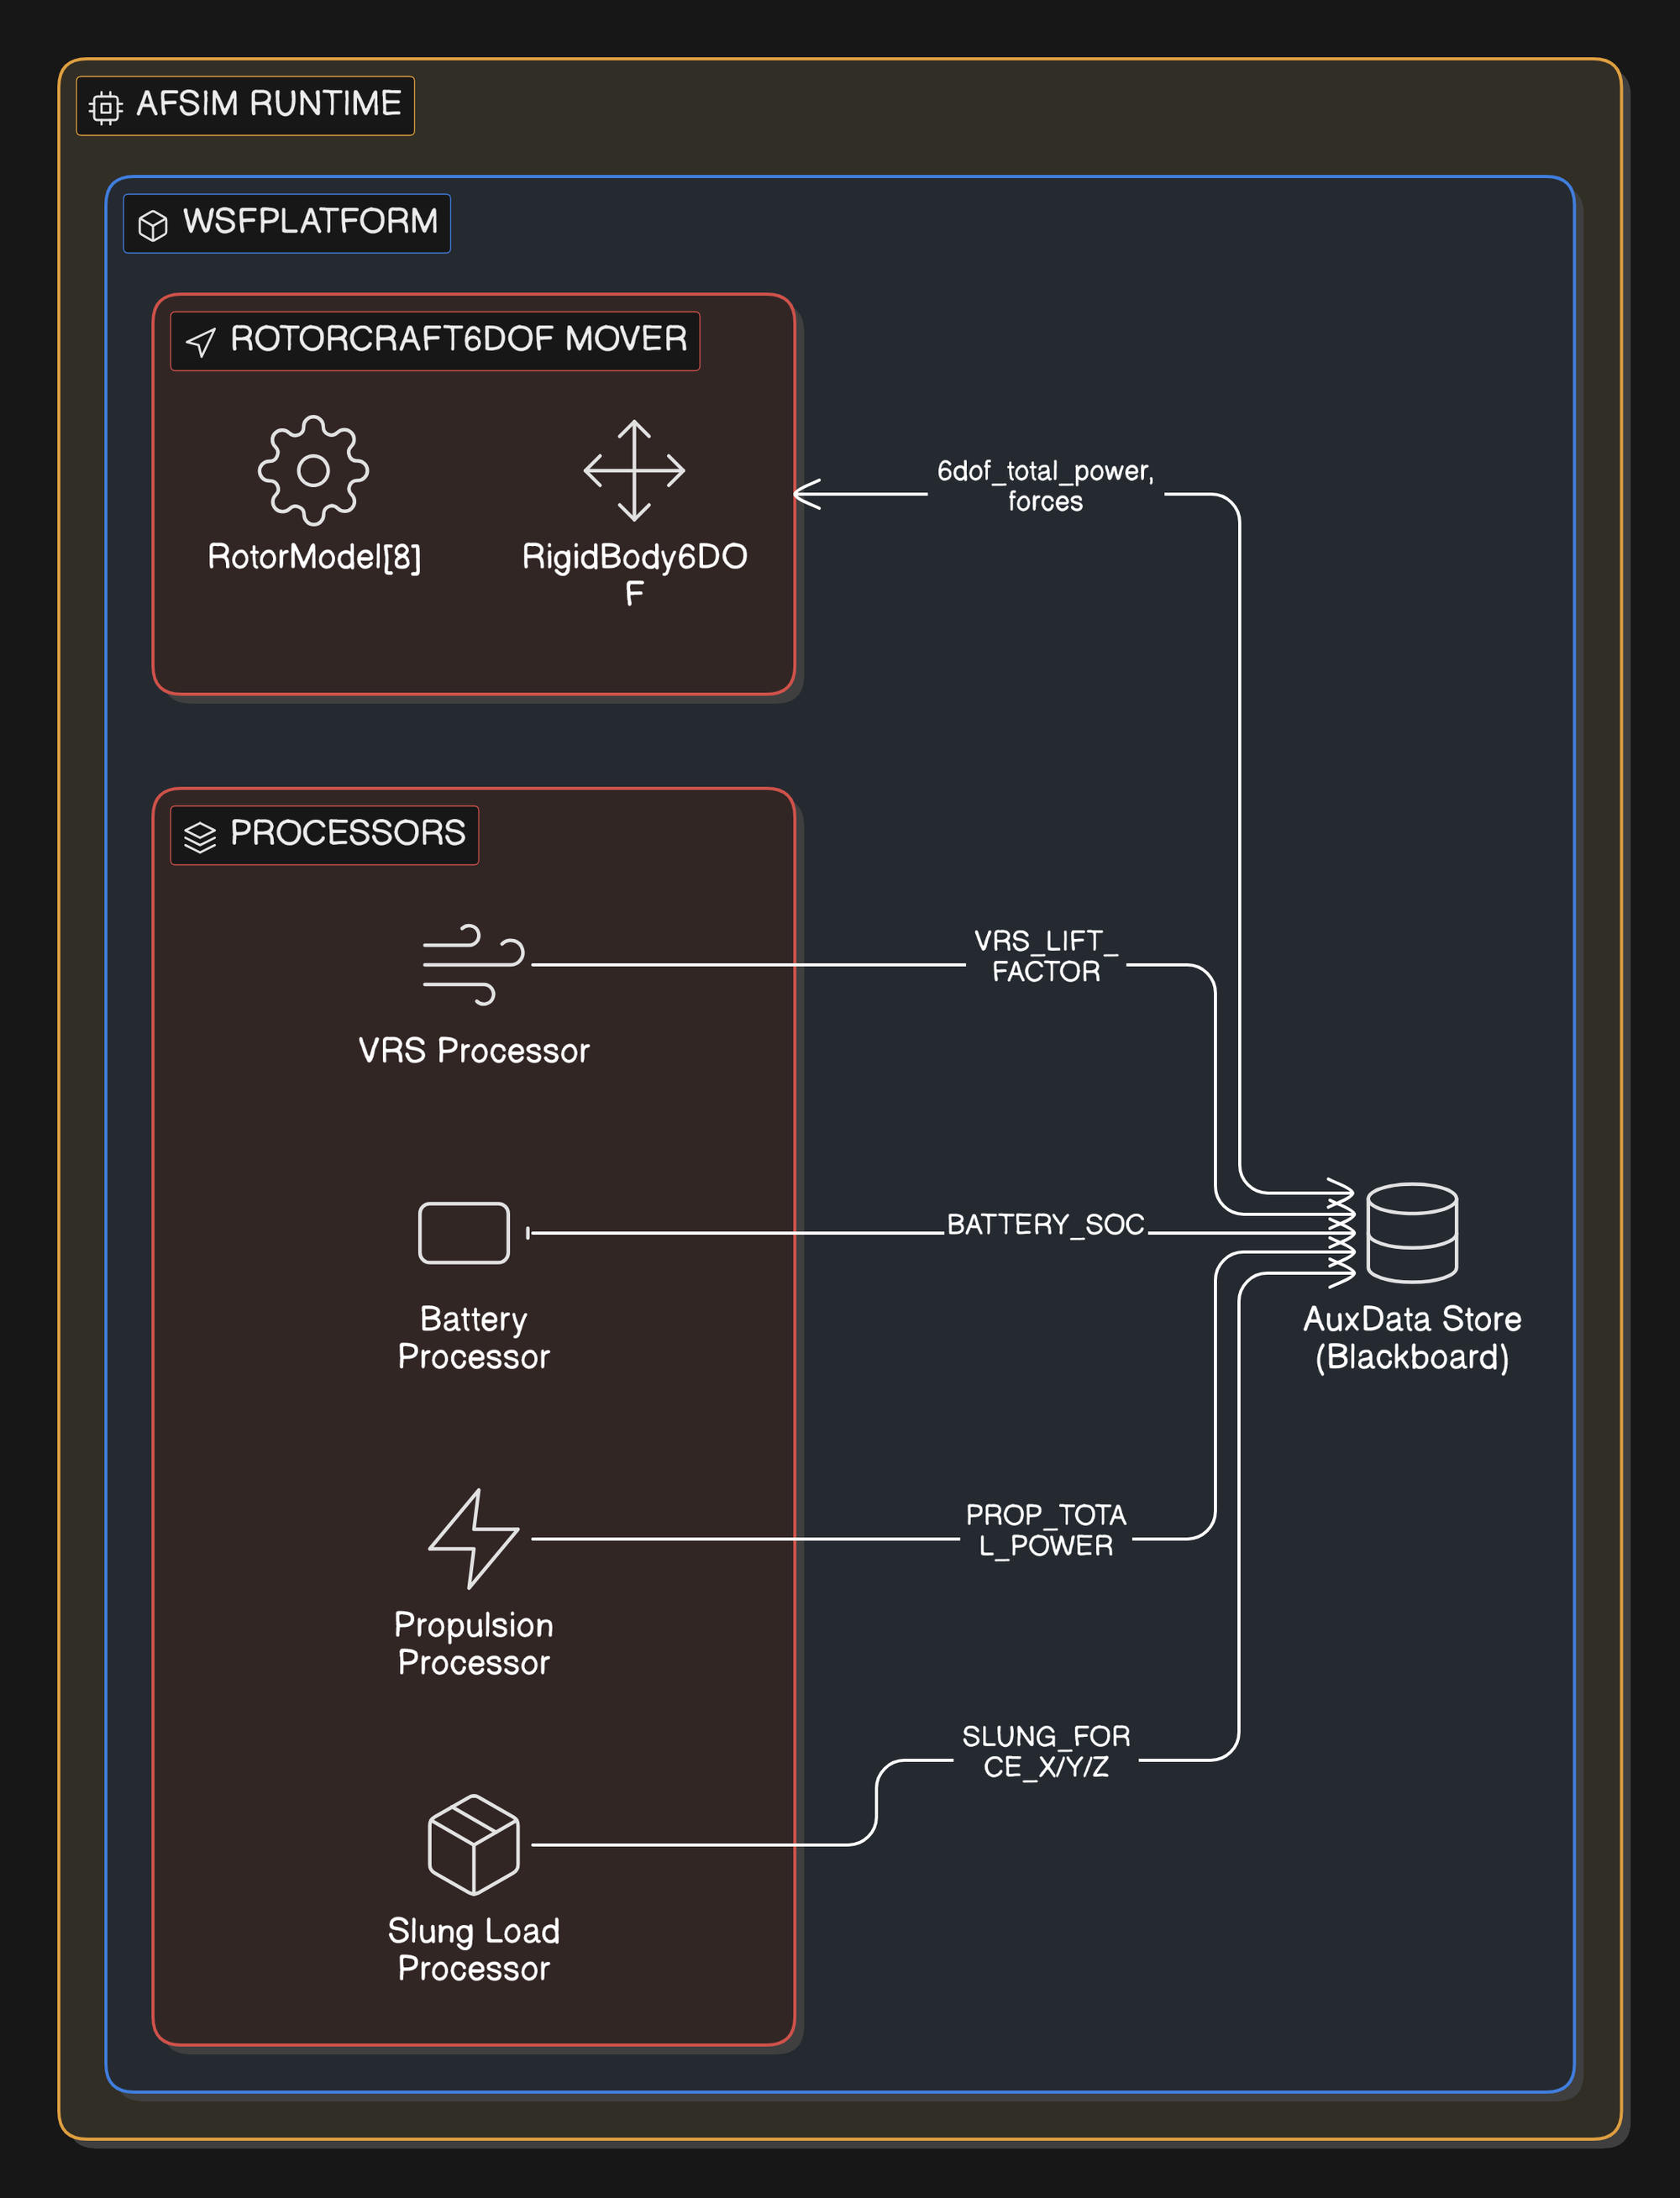
\includegraphics[width=\textwidth,height=0.85\textheight,keepaspectratio]{images/01_ADD_architecture_overview.png}
\caption{\unclass Architecture Overview}
\label{fig:architecture_overview}
\end{center}
\end{figure}

\unclass \textbf{Data flow direction}: Each processor writes its outputs to AuxData and reads its inputs from AuxData. The mover writes telemetry (position, velocity, thrust, power) and reads external forces (slung load, weapon recoil). The battery processor reads power from the propulsion processor or mover. This blackboard pattern ensures that any subset of plugins can operate without the others present.

\subsection{\unclass UML Class Diagram}\label{sec:UMLClassDiagram}

\begin{figure}[H]
\begin{center}
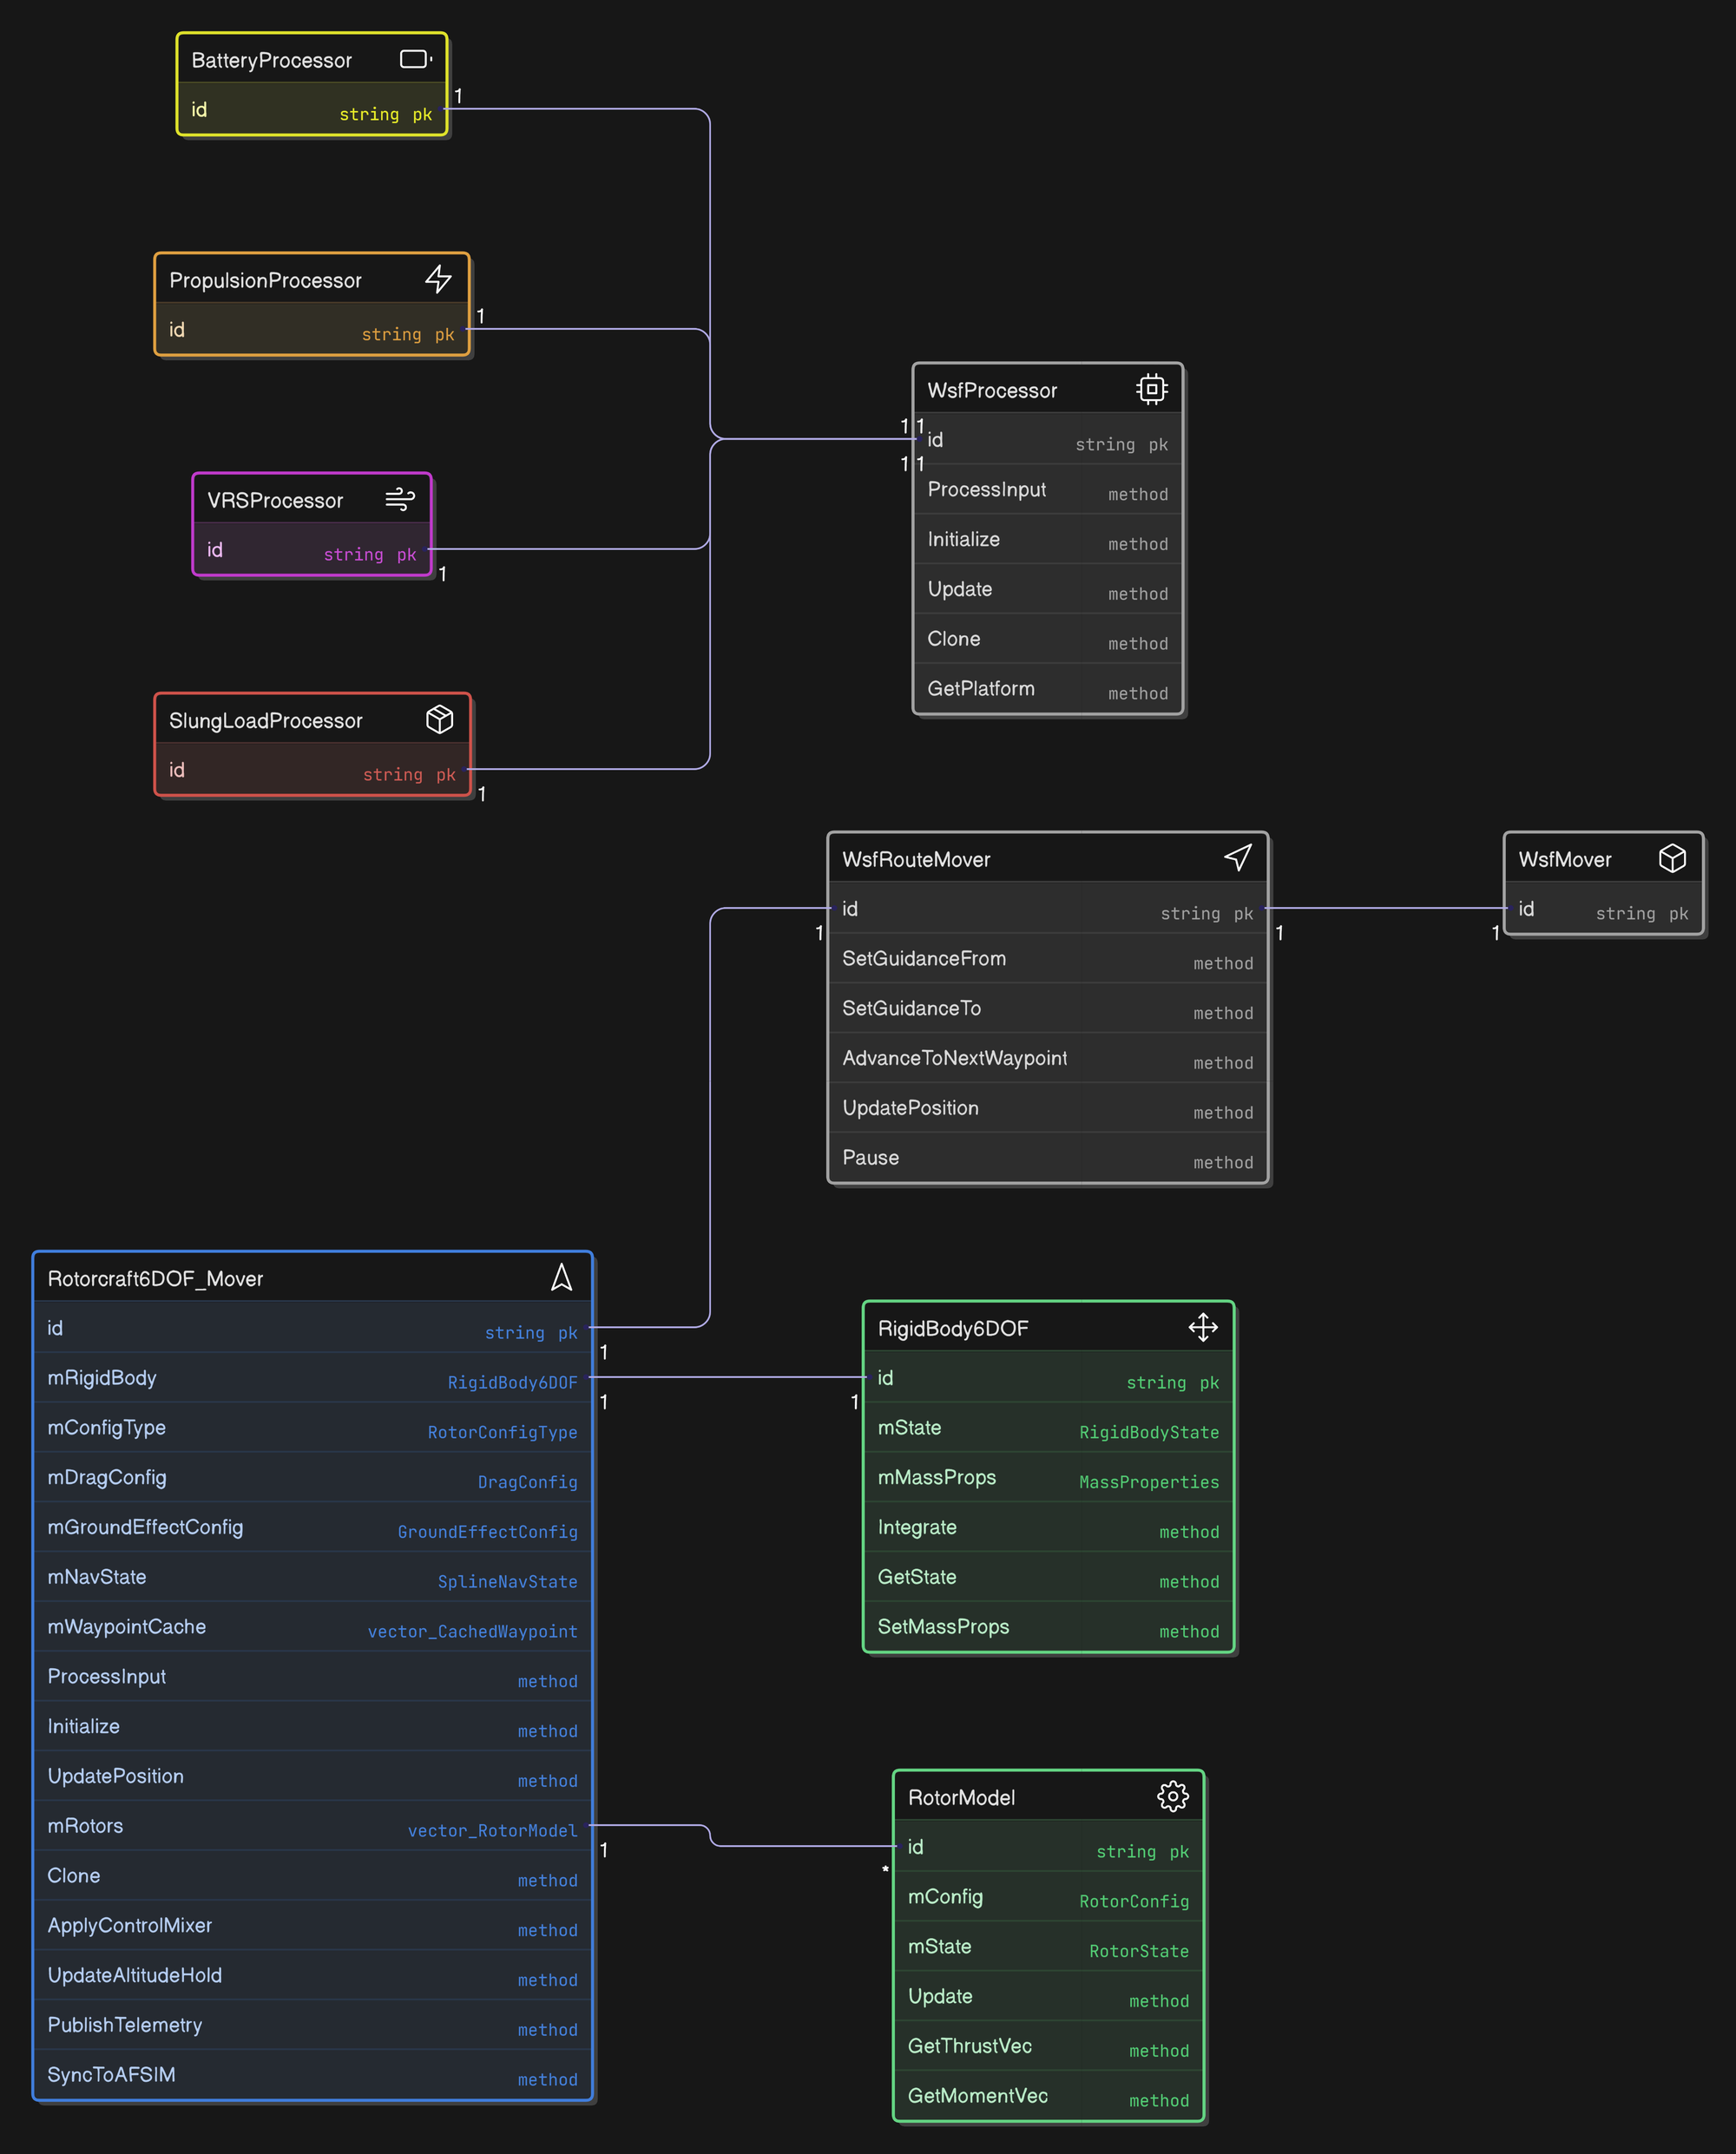
\includegraphics[width=\textwidth,height=0.85\textheight,keepaspectratio]{images/02_ADD_uml_class_hierarchy.png}
\caption{\unclass UML Class Hierarchy}
\label{fig:uml_class_hierarchy}
\end{center}
\end{figure}

\subsection{\unclass Plugin Registration Pattern}\label{sec:PluginRegistration}

\unclass All five plugins follow the same two-level registration pattern to register their types with AFSIM. This is the standard AFSIM plugin API contract.

\unclass \textbf{Registration sequence (pseudocode):}

\begin{figure}[H]
\begin{center}
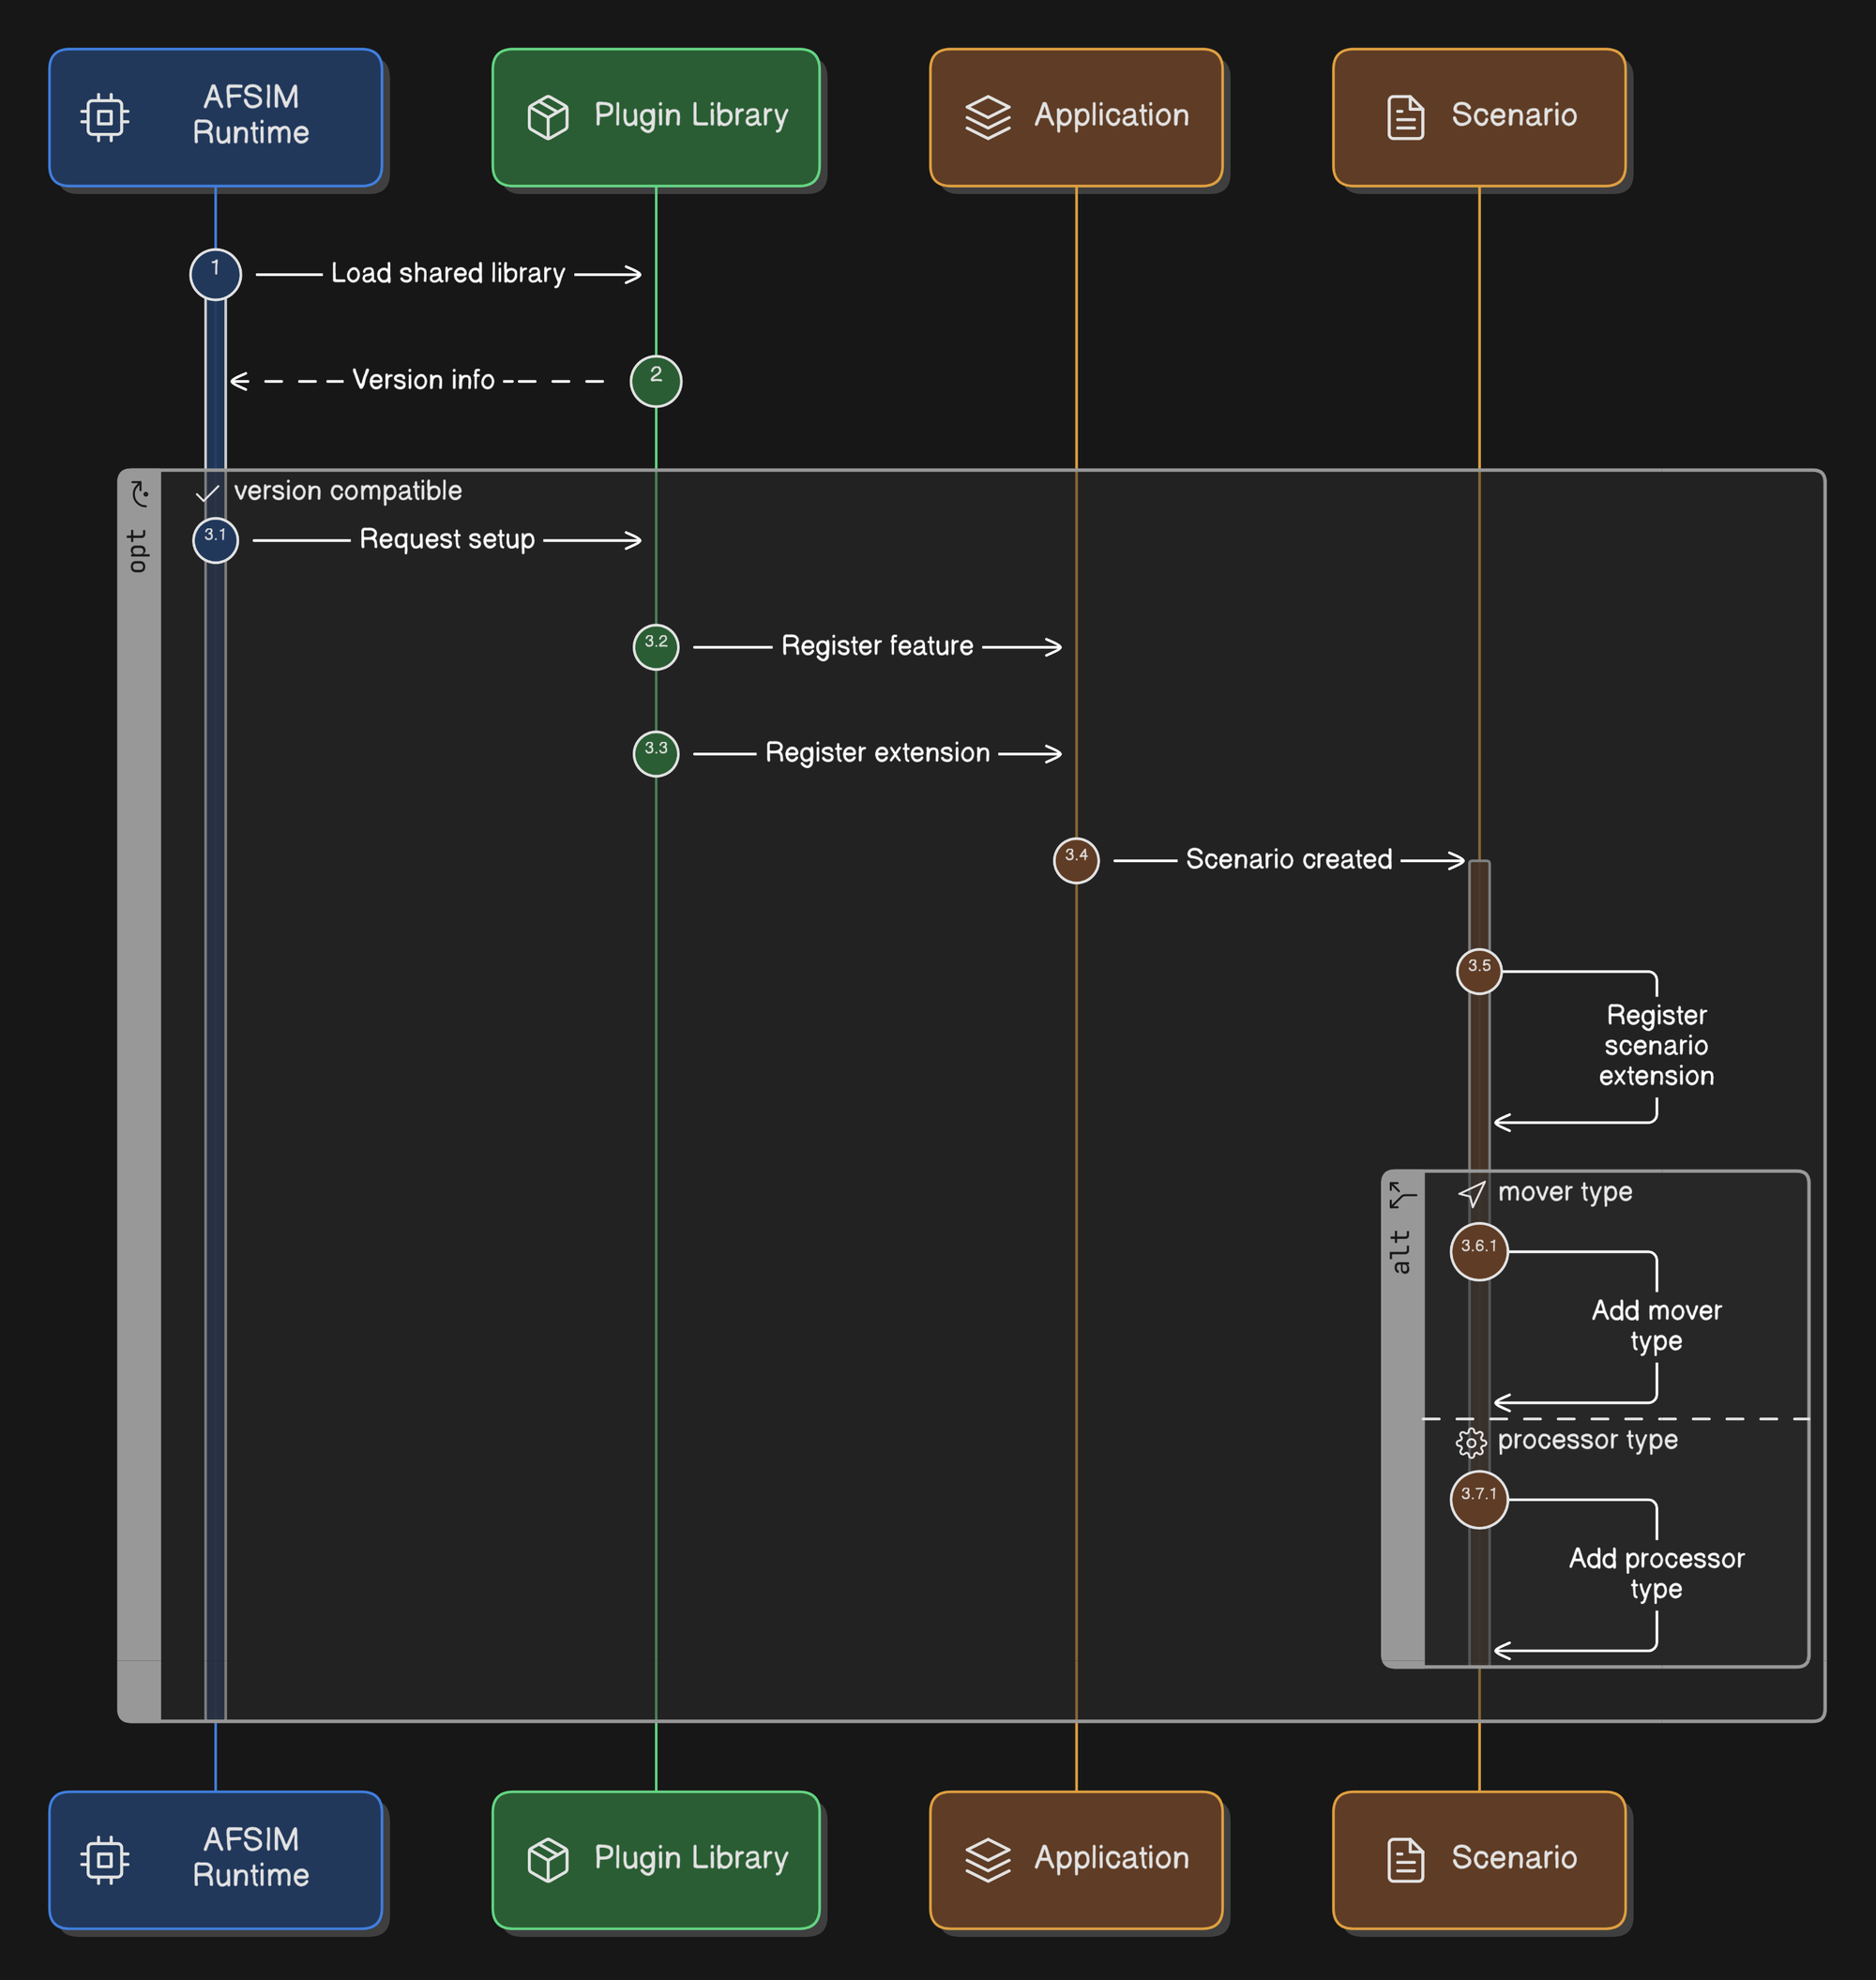
\includegraphics[width=\textwidth,height=0.85\textheight,keepaspectratio]{images/03_ADD_plugin_registration_sequence.png}
\caption{\unclass Plugin Registration Sequence}
\label{fig:plugin_registration_sequence}
\end{center}
\end{figure}

\unclass \textbf{Preconditions}: AFSIM must be initialized and the plugin shared library must be locatable via the plugin search path or scenario \texttt{plugin\_directory} directive.

\unclass \textbf{Expected outcomes}: After registration, the type name (e.g., \texttt{WSF\_ROTORCRAFT\_6DOF\_MOVER} or \texttt{T150\_BATTERY\_PROCESSOR}) becomes available for use in scenario files.

\unclass The 6DOF mover plugin uses the \texttt{WsfDefaultApplicationExtension} template helper, while the four processor plugins define a custom \texttt{ApplicationExtension} class with an identical pattern. Both approaches produce the same result: a \texttt{ScenarioExtension} is attached to each new scenario to register the plugin's type.

\subsection{\unclass Inter-Processor Communication via AuxData}\label{sec:AuxData}

\unclass Plugins communicate through the platform's \texttt{WsfAttributeContainer} (AuxData). Each plugin writes its outputs as named key-value pairs and reads inputs from keys published by other plugins. The following tables catalog all AuxData keys in the suite.

\subsubsection{\unclass Mover (Rotorcraft6DOF) -- Published Keys}

\tableThrNow{\unclasslabel}{\unclass Mover Published AuxData Keys}{MoverPublishedKeys}
{l,2in}{c,0.75in}{l,3in}
{
	Key & Type & Description \\
	\texttt{6dof\_pos\_n}, \texttt{\_e}, \texttt{\_d} & double & NED position [m] \\
	\texttt{6dof\_vel\_n}, \texttt{\_e}, \texttt{\_d} & double & NED velocity [m/s] \\
	\texttt{6dof\_roll\_deg}, \texttt{\_pitch\_deg}, \texttt{\_yaw\_deg} & double & Euler angles [deg] \\
	\texttt{6dof\_p\_dps}, \texttt{\_q\_dps}, \texttt{\_r\_dps} & double & Angular rates [deg/s] \\
	\texttt{6dof\_total\_thrust} & double & Sum of all rotor thrust [N] \\
	\texttt{6dof\_total\_power} & double & Sum of all rotor power [W] \\
	\texttt{6dof\_throttle\_cmd} & double & Throttle command [0--1] \\
	\texttt{6dof\_avg\_rpm} & double & Average rotor RPM \\
	\texttt{6dof\_mass}, \texttt{6dof\_weight} & double & Current mass [kg], weight [N] \\
}

\subsubsection{\unclass Mover (Rotorcraft6DOF) -- Read Keys}

\tableThrNow{\unclasslabel}{\unclass Mover Read AuxData Keys}{MoverReadKeys}
{l,2in}{l,1.5in}{l,2.5in}
{
	Key & Source Plugin & Description \\
	\texttt{SLUNG\_FORCE\_X/Y/Z} & SlungLoadProcessor & Cable reaction forces [N] \\
	\texttt{WEAPON\_FORCE\_X/Y/Z} & WeaponProcessor & Recoil forces [N] \\
	\texttt{WEAPON\_MOMENT\_X/Y/Z} & WeaponProcessor & Recoil moments [Nm] \\
	\texttt{WEAPON\_REGISTRY} & WeaponProcessor & Comma-separated weapon names \\
	\texttt{WEAPON\_<name>\_MASS\_DELTA} & WeaponProcessor & Ammunition mass change [kg] \\
	\texttt{SLUNG\_LOAD\_STATE} & SlungLoadProcessor & Load state enumeration \\
	\texttt{SLUNG\_LOAD\_MASS} & SlungLoadProcessor & Load mass for dynamic mass update [kg] \\
}

\subsubsection{\unclass BatteryProcessor -- Published Keys}

\tableThrNow{\unclasslabel}{\unclass Battery Published AuxData Keys}{BatteryPublishedKeys}
{l,2in}{c,0.75in}{l,3in}
{
	Key & Type & Description \\
	\texttt{BATTERY\_SOC} & double & State of charge [0--1] \\
	\texttt{BATTERY\_POWER\_W} & double & Current power draw [W] \\
	\texttt{BATTERY\_ENERGY\_WH} & double & Remaining energy [Wh] \\
	\texttt{BATTERY\_VOLTAGE} & double & Terminal voltage [V] \\
	\texttt{BATTERY\_OCV} & double & Open-circuit voltage [V] \\
	\texttt{BATTERY\_VOLTAGE\_SAG} & double & Voltage drop from internal resistance [V] \\
	\texttt{BATTERY\_CURRENT\_A} & double & Pack current [A] \\
	\texttt{BATTERY\_LOW} & bool & Low SOC warning flag \\
	\texttt{BATTERY\_VOLTAGE\_LOW} & bool & Voltage sag warning flag \\
}

\subsubsection{\unclass BatteryProcessor -- Read Keys}

\tableThrNow{\unclasslabel}{\unclass Battery Read AuxData Keys}{BatteryReadKeys}
{l,2in}{l,1.5in}{l,2.5in}
{
	Key & Source Plugin & Description \\
	\texttt{PROP\_TOTAL\_POWER} & PropulsionProcessor & Propulsion power [W] (primary source) \\
	\texttt{6dof\_total\_power} & Rotorcraft6DOF Mover & Mover power [W] (fallback source) \\
}

\subsubsection{\unclass PropulsionProcessor -- Published Keys}

\tableThrNow{\unclasslabel}{\unclass Propulsion Published AuxData Keys}{PropPublishedKeys}
{l,2in}{c,0.75in}{l,3in}
{
	Key & Type & Description \\
	\texttt{PROP\_TOTAL\_THRUST} & double & Total thrust [N] \\
	\texttt{PROP\_TOTAL\_POWER} & double & Total electrical power [W] \\
	\texttt{PROP\_SYSTEM\_EFF} & double & System efficiency [0--1] \\
	\texttt{PROP\_MOTOR\_COUNT} & int & Operational motor count \\
	\texttt{PROP\_GROUND\_EFFECT} & double & Ground effect multiplier \\
	\texttt{PROP\_ALTITUDE\_AGL} & double & Altitude AGL [m] \\
	\texttt{PROP\_TOTAL\_MASS} & double & Total mass [kg] \\
	\texttt{PROP\_PAYLOAD\_MASS} & double & Payload mass [kg] \\
	\texttt{PROP\_THRUST\_MARGIN} & double & Available thrust margin [0--1] \\
	\texttt{PROP\_CG\_OFFSET\_X/Y/Z} & double & Combined CG offset [m] \\
	\texttt{PROP\_FORWARD\_SPEED} & double & Horizontal speed [m/s] \\
	\texttt{PROP\_CLIMB\_RATE} & double & Vertical speed [m/s] \\
	\texttt{PROP\_BANK\_ANGLE} & double & Bank angle [deg] \\
	\texttt{PROP\_OVERLOADED} & bool & Payload exceeds capacity \\
	\texttt{MOTOR\_OVERTEMP} & bool & Motor over-temperature flag \\
	\texttt{MOTOR\_FAILURE} & bool & Motor failure flag \\
}

\subsubsection{\unclass VRSProcessor -- Published Keys}

\tableThrNow{\unclasslabel}{\unclass VRS Published AuxData Keys}{VRSPublishedKeys}
{l,2in}{c,0.75in}{l,3in}
{
	Key & Type & Description \\
	\texttt{VRS\_MARGIN} & double & VRS proximity margin [0--1] \\
	\texttt{VRS\_STATE} & int & VRS state enumeration \\
	\texttt{VRS\_LIFT\_FACTOR} & double & Lift degradation factor [0--1] \\
	\texttt{VRS\_CONTROL\_FACTOR} & double & Control authority factor [0--1] \\
	\texttt{VRS\_DEVELOPMENT} & double & VRS development level [0--1] \\
	\texttt{VRS\_DESCENT\_RATE} & double & Current descent rate [m/s] \\
	\texttt{VRS\_FORWARD\_SPEED} & double & Current forward speed [m/s] \\
	\texttt{VRS\_CAUTION}, \texttt{\_ONSET}, \texttt{\_CRITICAL} & bool & Warning flags \\
}

\subsubsection{\unclass SlungLoadProcessor -- Published Keys}

\tableThrNow{\unclasslabel}{\unclass Slung Load Published AuxData Keys}{SlungPublishedKeys}
{l,2in}{c,0.75in}{l,3in}
{
	Key & Type & Description \\
	\texttt{SLUNG\_LOAD\_STATE} & int & Load state enumeration \\
	\texttt{SLUNG\_LOAD\_MASS} & double & Load mass [kg] \\
	\texttt{SLUNG\_CABLE\_LENGTH} & double & Cable length [m] \\
	\texttt{SLUNG\_CABLE\_TENSION} & double & Cable tension [N] \\
	\texttt{SLUNG\_SWING\_X}, \texttt{\_Y} & double & Swing angles [deg] \\
	\texttt{SLUNG\_SWING\_MAG} & double & Swing magnitude [deg] \\
	\texttt{SLUNG\_FORCE\_X/Y/Z} & double & Reaction forces on aircraft [N] \\
	\texttt{SLUNG\_POS\_X/Y/Z} & double & Load position relative to CG [m] \\
	\texttt{SLUNG\_RESONANCE} & bool & Resonance warning flag \\
	\texttt{SLUNG\_NATURAL\_FREQ} & double & Pendulum natural frequency [Hz] \\
}

\pagebreak

%%%%%%%%%%%%%%%%%%%%%%%%%%%%%%%%%%%%%%%%%%%%%%%%%%%%%%%%%%%%
%% SECTION 3: Component -- Rotorcraft6DOF Mover
%%%%%%%%%%%%%%%%%%%%%%%%%%%%%%%%%%%%%%%%%%%%%%%%%%%%%%%%%%%%

\section{\unclass Component: Rotorcraft6DOF Mover}\label{sec:Rotorcraft6DOF}

\subsection{\unclass Structural Overview}\label{sec:6DOFOverview}

\unclass The Rotorcraft6DOF Mover is the core flight dynamics component. It extends \texttt{WsfRouteMover} (which itself extends \texttt{WsfMover}) to inherit route/waypoint navigation integration while replacing the position update logic with full 6DOF physics.

\unclass \textbf{Source files:}

\tableThrNow{\unclasslabel}{\unclass Rotorcraft6DOF Source Files}{6DOFSourceFiles}
{l,2.5in}{l,2.5in}{c,0.75in}
{
	File & Purpose & LOC \\
	\texttt{Rotorcraft6DOF\_Mover.hpp} & Class declaration, enums, structs & 489 \\
	\texttt{Rotorcraft6DOF\_Mover.cpp} & Implementation & $\sim$2,450 \\
	\texttt{RigidBody6DOF.hpp} & Rigid body state and integrator & 214 \\
	\texttt{RigidBody6DOF.cpp} & Integration implementation & $\sim$150 \\
	\texttt{RotorModel.hpp} & Single rotor model & 181 \\
	\texttt{RotorModel.cpp} & Rotor physics implementation & $\sim$120 \\
	\texttt{MathUtils.hpp} & Vector3, Quaternion, Matrix3x3, spline math & 511 \\
	\texttt{Rotorcraft6DOF\_Registration.hpp} & Scenario extension & 56 \\
	\texttt{Rotorcraft6DOF\_PluginRegistration.cpp} & Plugin entry points & 57 \\
}

\unclass \textbf{Namespace}: \texttt{rotorcraft\_6dof}

\subsection{\unclass Composition Structure}\label{sec:6DOFComposition}

\unclass The mover contains the following owned objects:

\begin{itemize}
	\item \unclass \textbf{RigidBody6DOF} (\texttt{mRigidBody}) -- Holds the kinematic state (position, velocity, orientation quaternion, angular velocity) and mass properties. Provides the \texttt{Integrate()} method that advances state by one timestep given total forces and moments.
	\item \unclass \textbf{vector\textless RotorModel\textgreater} (\texttt{mRotors}) -- Array of N rotor models, sized by configuration (4 for QUAD, 8 for COAXIAL\_QUAD). Each rotor independently computes thrust, torque, and power from its commanded RPM.
	\item \unclass \textbf{DragConfig} (\texttt{mDragConfig}) -- Aerodynamic drag coefficients and reference area.
	\item \unclass \textbf{GroundEffectConfig} (\texttt{mGroundEffectConfig}) -- Ground effect parameters.
	\item \unclass \textbf{map\textless int, WaypointConfig\textgreater} (\texttt{mWaypointConfigs}) -- Per-waypoint behavior overrides for spline navigation.
	\item \unclass \textbf{vector\textless CachedWaypoint\textgreater} (\texttt{mWaypointCache}) -- Sliding window of four waypoints for Catmull-Rom spline interpolation.
\end{itemize}

\subsection{\unclass WsfRouteMover Interface}\label{sec:RouteMoverInterface}

\unclass The mover implements the pure virtual methods required by \texttt{WsfRouteMover}:

\tableTwoNow{\unclasslabel}{\unclass WsfRouteMover Interface Methods}{RouteMoverMethods}{l,2in}{l,4in}{
	Method & Behavior \\
	\texttt{SetGuidanceFrom(waypoint)} & Caches the previous waypoint for speed reference. \\
	\texttt{SetGuidanceTo(waypoint)} & Sets target altitude and speed from the next waypoint. \\
	\texttt{AdvanceToNextWaypoint(time, target, next)} & Configures guidance for the next segment. If spline navigation is enabled, advances the waypoint cache and recomputes the speed profile. \\
	\texttt{UpdatePosition(simTime)} & Core physics loop -- computes forces, integrates rigid body, synchronizes AFSIM platform state. \\
	\texttt{Pause(simTime, unpauseTime)} & Enters hover-hold at current position until \texttt{unpauseTime}. \\
}

\subsection{\unclass UpdatePosition Sequence}\label{sec:UpdatePositionSeq}

\unclass The \texttt{UpdatePosition()} method executes the following sequence each timestep:

\begin{figure}[H]
\begin{center}
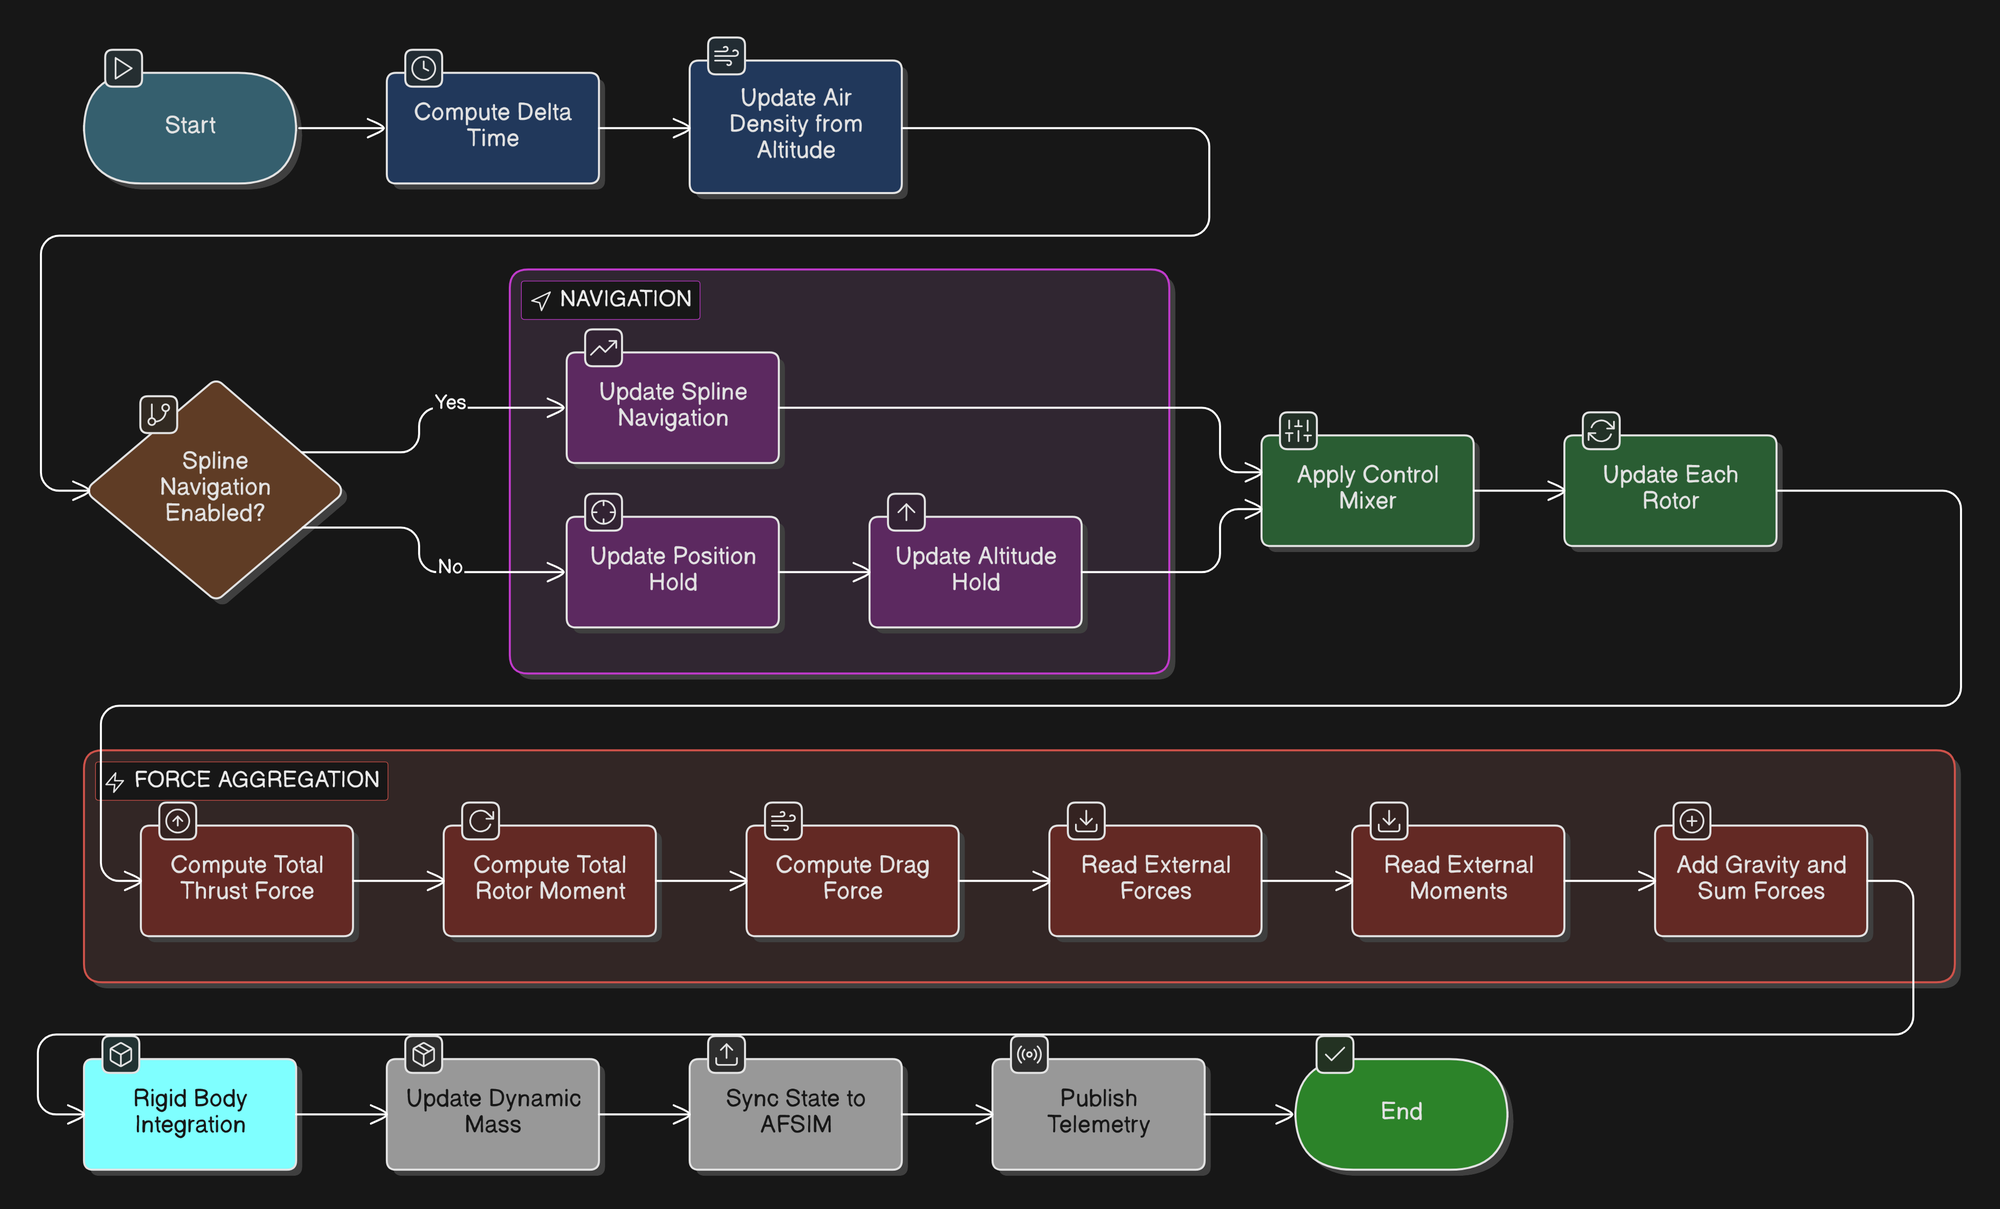
\includegraphics[width=\textwidth,height=0.85\textheight,keepaspectratio]{images/04_ADD_update_position_sequence.png}
\caption{\unclass UpdatePosition Sequence}
\label{fig:update_position_sequence}
\end{center}
\end{figure}

\subsection{\unclass Spline Navigation State Machine}\label{sec:SplineNavStateMachine}

\unclass When spline navigation is enabled, the mover uses a Catmull-Rom spline interpolation across a sliding window of four cached waypoints (P0, P1, P2, P3) to produce smooth flight paths. The navigation state machine governs behavior at each waypoint.

\begin{figure}[H]
\begin{center}
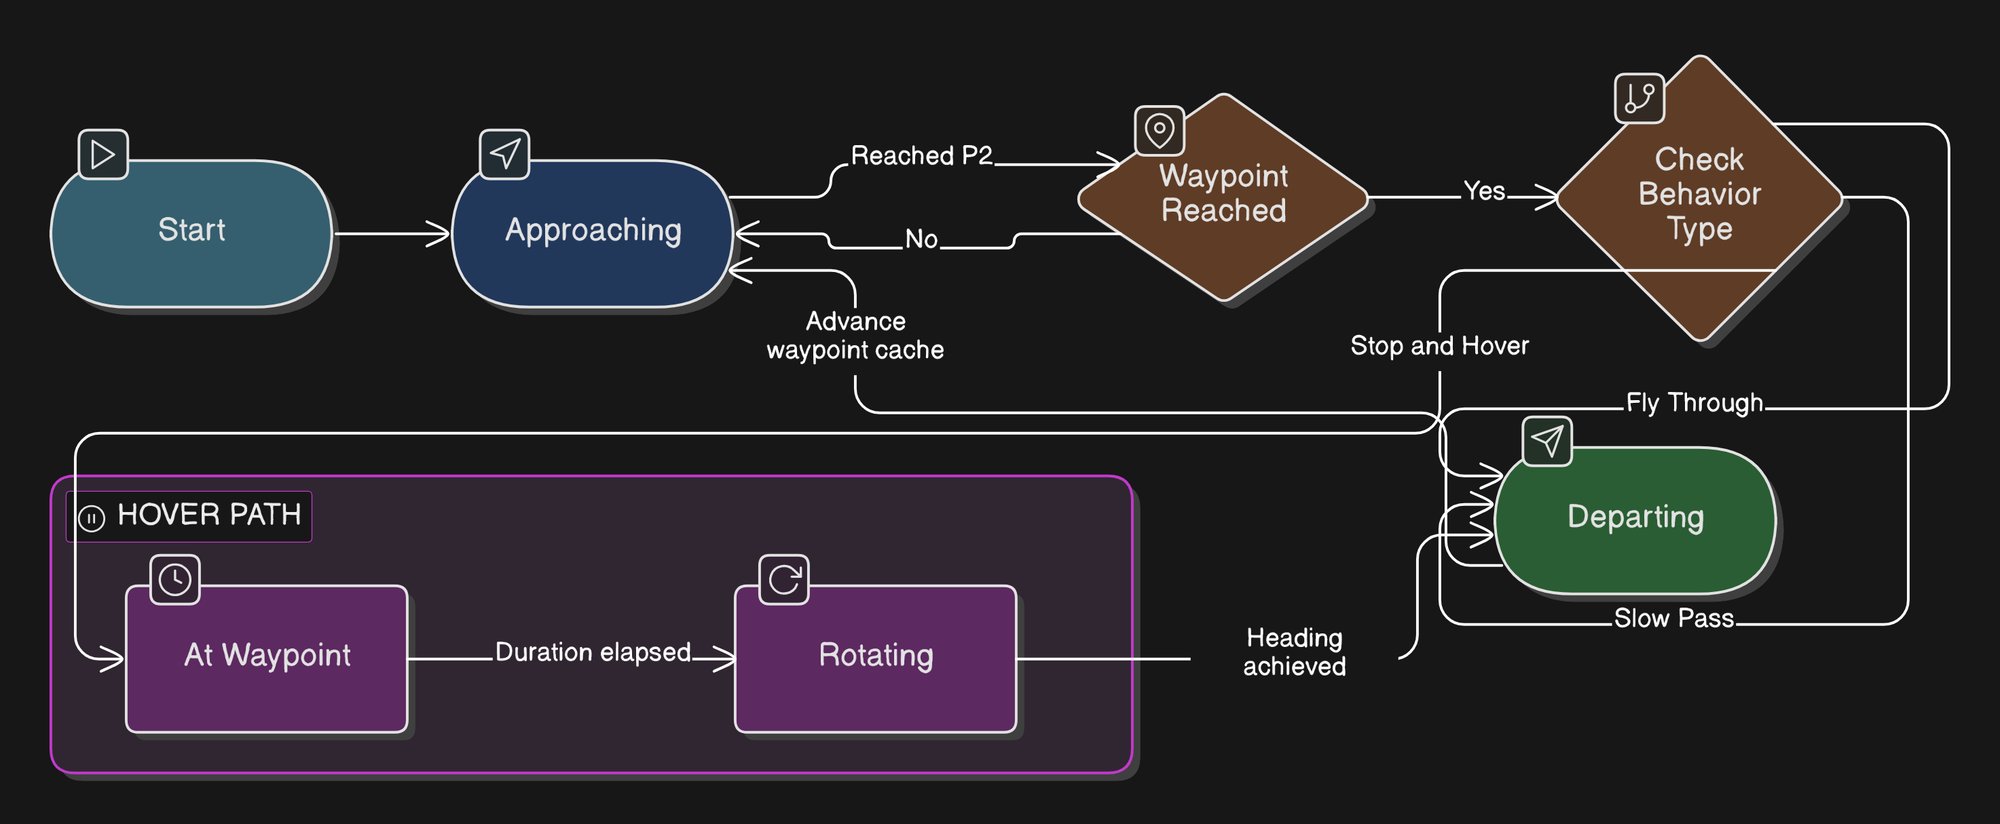
\includegraphics[width=0.8\textwidth,height=0.85\textheight,keepaspectratio]{images/05_ADD_spline_navigation_state_machine.png}
\caption{\unclass Spline Navigation State Machine}
\label{fig:spline_navigation_state_machine}
\end{center}
\end{figure}

\unclass \textbf{State descriptions:}

\tableFouNow{\unclasslabel}{\unclass Spline Navigation States}{SplineNavStates}
{l,1.2in}{l,1.5in}{l,2in}{l,1.5in}
{
	State & Precondition & Behavior & Exit Condition \\
	APPROACHING & Waypoint cache initialized & Follow spline toward P2 at profiled speed & Distance to P2 $<$ arrival radius \\
	AT\_WAYPOINT & STOP\_AND\_HOVER behavior & Hold position, zero velocity & Hover duration elapsed \\
	ROTATING & Departure heading specified & Yaw to face next waypoint & Heading error $<$ threshold \\
	DEPARTING & Rotation complete or FLY\_THROUGH & Advance waypoint cache, accelerate & Spline parameter reset, transition to APPROACHING \\
}

\subsection{\unclass Rotor Configuration System}\label{sec:RotorConfig}

\unclass The mover supports multiple rotor configurations through the \texttt{RotorConfigType} enumeration:

\tableFouNow{\unclasslabel}{\unclass Rotor Configurations}{RotorConfigs}
{l,1.5in}{c,0.75in}{c,0.5in}{l,2.5in}
{
	Configuration & Rotors & Arms & Description \\
	\texttt{QUAD\_X} & 4 & 4 & X-pattern quadcopter \\
	\texttt{QUAD\_PLUS} & 4 & 4 & Plus-pattern quadcopter \\
	\texttt{HEX\_X} & 6 & 6 & Hexacopter \\
	\texttt{OCTO\_X} & 8 & 8 & Flat octocopter \\
	\texttt{COAXIAL\_QUAD} & 8 & 4 & Coaxial quadcopter (T-150 default) \\
	\texttt{COAXIAL\_OCTO} & 16 & 8 & Coaxial octocopter \\
	\texttt{CUSTOM} & N & N & User-defined rotor positions \\
}

\unclass Each \texttt{Setup*()} method populates the \texttt{mRotors} vector with \texttt{RotorModel} instances whose \texttt{RotorConfig} specifies body-frame position, rotation direction (CW/CCW), thrust axis, and control mixing factors (roll, pitch, yaw).

\subsection{\unclass Public Interface Summary}\label{sec:6DOFPublicInterface}

\tableThrNow{\unclasslabel}{\unclass Rotorcraft6DOF Public Interface}{6DOFPublicInterface}
{l,2in}{l,1.5in}{l,2.5in}
{
	Method & Precondition & Expected Outcome \\
	\texttt{ProcessInput(input)} & Scenario file parsed & Configuration loaded: mass, rotors, gains, spline settings \\
	\texttt{Initialize(simTime)} & ProcessInput complete & 6DOF state initialized from AFSIM platform position, hover RPM computed \\
	\texttt{UpdatePosition(simTime)} & Initialize complete & Platform position/velocity/attitude advanced by one timestep \\
	\texttt{SetRotorConfigType(type)} & Before Initialize & Rotor array populated with preset geometry \\
	\texttt{GetTotalThrust()} & Any time after Initialize & Returns sum of all rotor thrust values [N] \\
	\texttt{GetTotalPower()} & Any time after Initialize & Returns sum of all rotor power values [W] \\
}

\pagebreak

%%%%%%%%%%%%%%%%%%%%%%%%%%%%%%%%%%%%%%%%%%%%%%%%%%%%%%%%%%%%
%% SECTION 4: Component -- BatteryProcessor
%%%%%%%%%%%%%%%%%%%%%%%%%%%%%%%%%%%%%%%%%%%%%%%%%%%%%%%%%%%%

\section{\unclass Component: BatteryProcessor}\label{sec:BatteryProcessor}

\subsection{\unclass Structural Overview}\label{sec:BatteryOverview}

\unclass The BatteryProcessor models a lithium-ion battery pack, tracking state-of-charge (SOC), terminal voltage under load, and energy consumption. It extends \texttt{WsfProcessor} and follows the standard ProcessInput/Initialize/Update lifecycle.

\unclass \textbf{Source files:}

\tableTwoNow{\unclasslabel}{\unclass Battery Source Files}{BatterySourceFiles}{l,2.5in}{l,3in}{
	File & Purpose \\
	\texttt{BatteryProcessor.hpp} & Class declaration \\
	\texttt{BatteryProcessor.cpp} & Implementation \\
	\texttt{BatteryRegistration.hpp} & Scenario extension \\
	\texttt{BatteryPluginRegistration.cpp} & Plugin entry points \\
}

\unclass \textbf{Namespace}: \texttt{t150}

\subsection{\unclass Lifecycle}\label{sec:BatteryLifecycle}

\begin{figure}[H]
\begin{center}
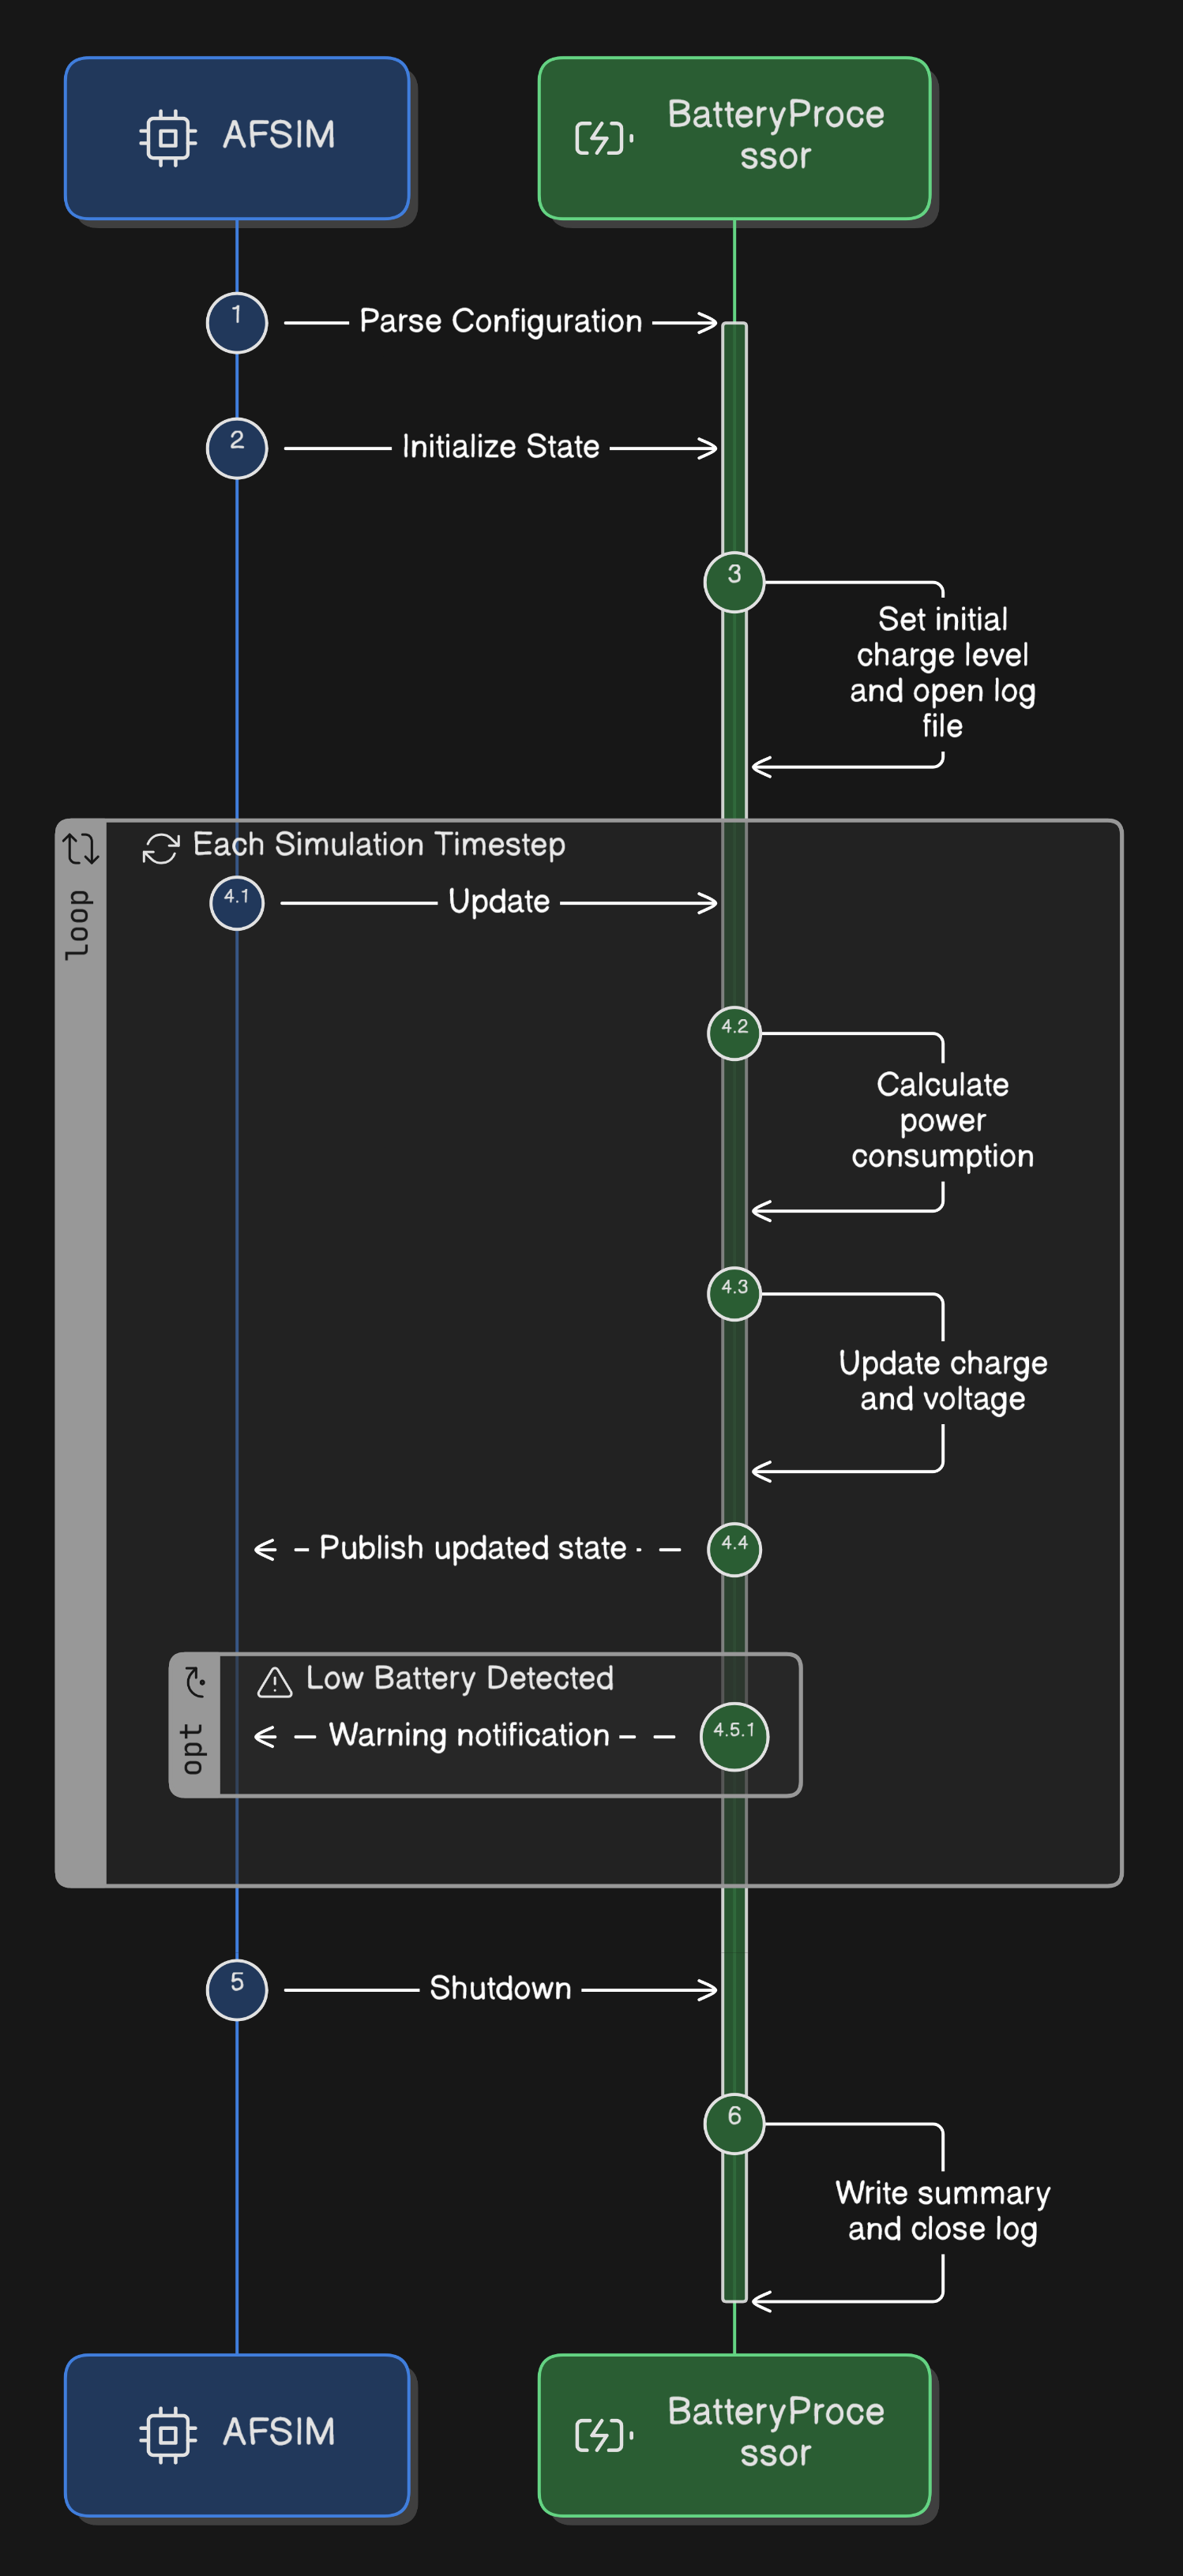
\includegraphics[width=\textwidth,height=0.85\textheight,keepaspectratio]{images/06_ADD_battery_lifecycle_sequence.png}
\caption{\unclass Battery Processor Lifecycle Sequence}
\label{fig:battery_lifecycle_sequence}
\end{center}
\end{figure}

\subsection{\unclass Power Source Resolution}\label{sec:PowerSourceResolution}

\unclass The battery processor reads power consumption through a configurable AuxData key. The resolution order provides fallback behavior:

\begin{figure}[H]
\begin{center}
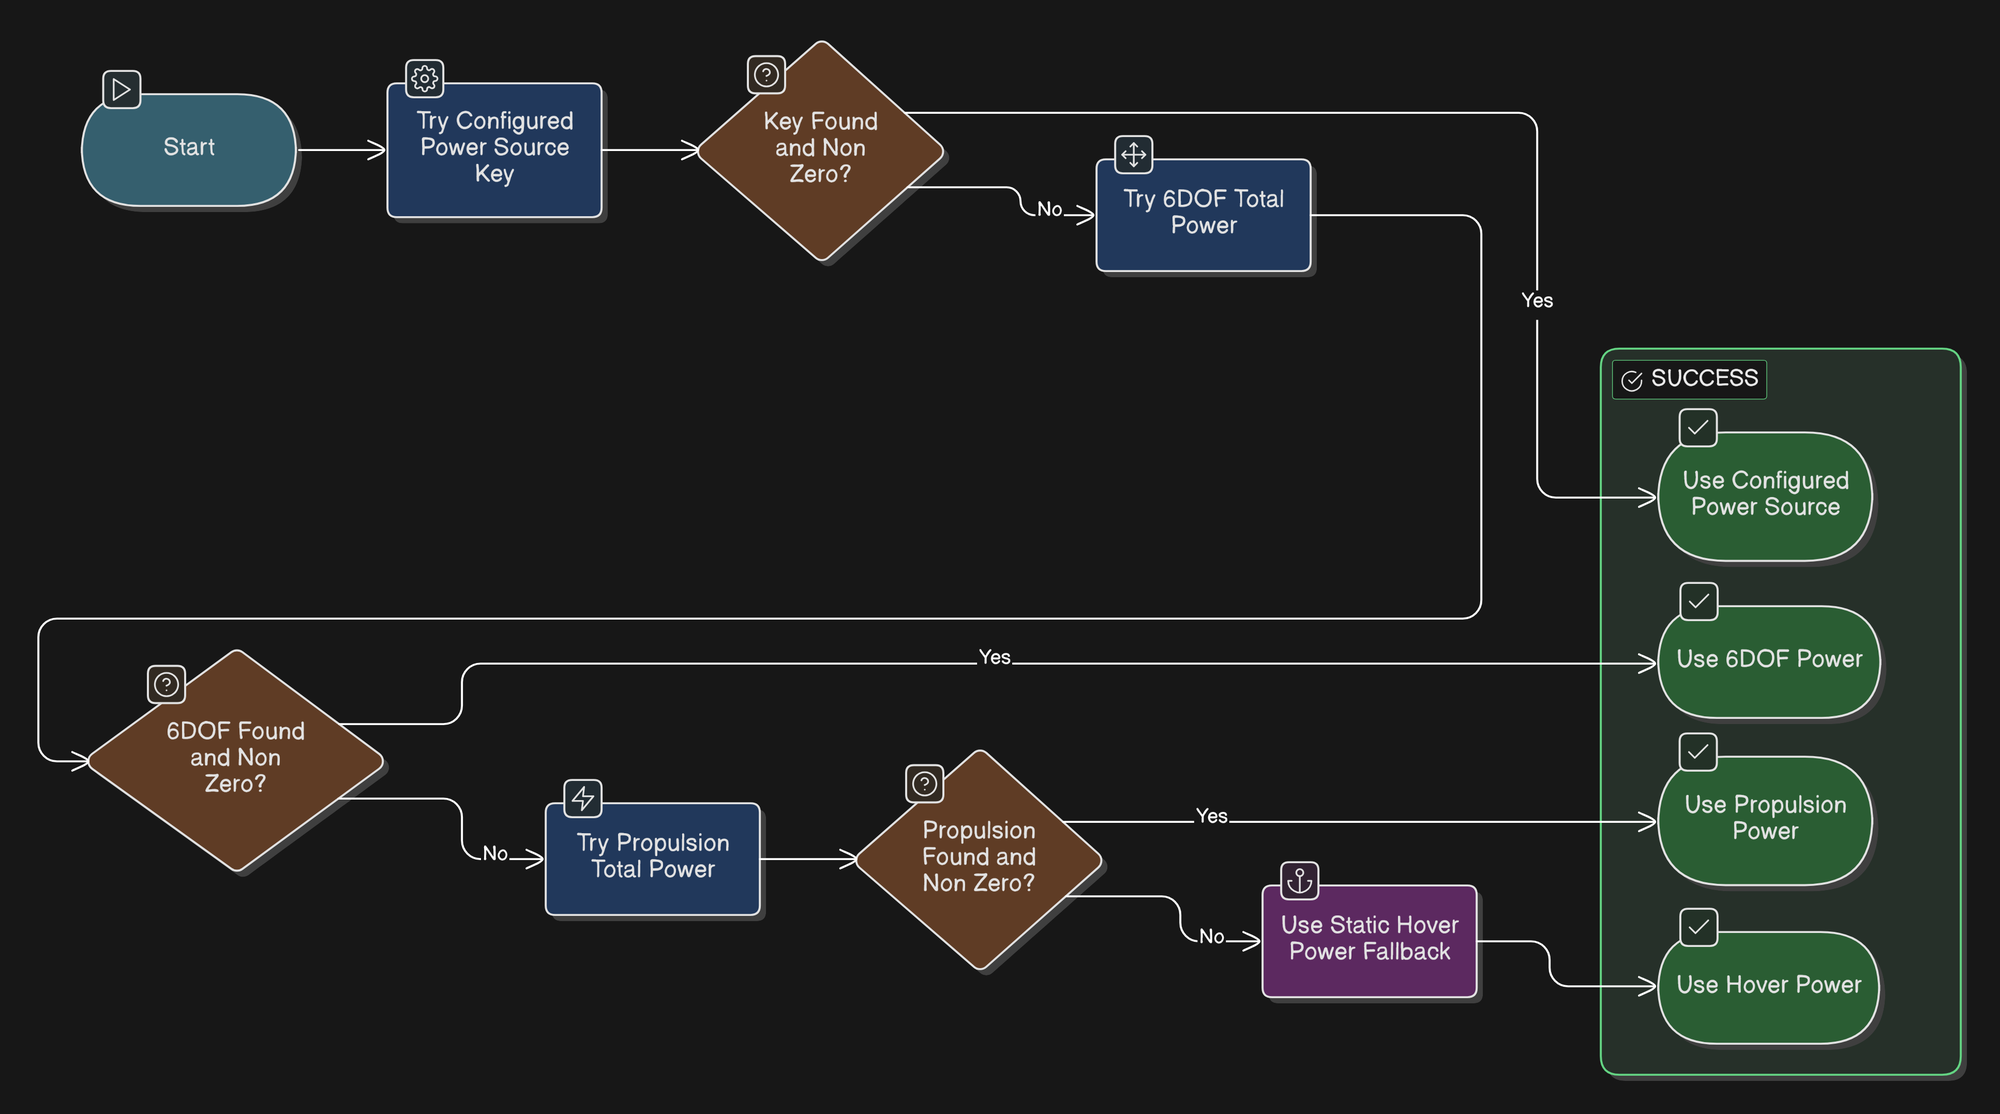
\includegraphics[width=0.8\textwidth,height=0.85\textheight,keepaspectratio]{images/07_ADD_power_source_resolution.png}
\caption{\unclass Power Source Resolution}
\label{fig:power_source_resolution}
\end{center}
\end{figure}

\unclass This cascade ensures the battery processor functions regardless of which other plugins are loaded.

\subsection{\unclass Voltage Sag Solver}\label{sec:VoltageSagSolver}

\unclass The terminal voltage under load is computed by solving for the current that satisfies both:
\begin{itemize}
	\item $V_{terminal} = V_{oc} - I \cdot R_{internal}$
	\item $P = V_{terminal} \cdot I$
\end{itemize}

\unclass Substituting yields a quadratic in voltage. The processor selects the physically meaningful root (higher voltage). If the quadratic has no real roots (power demand exceeds what the battery can deliver), the terminal voltage is clamped to the cutoff voltage.

\subsection{\unclass Public Interface Summary}\label{sec:BatteryPublicInterface}

\tableThrNow{\unclasslabel}{\unclass BatteryProcessor Public Interface}{BatteryPublicInterface}
{l,2in}{l,1.5in}{l,2.5in}
{
	Method & Precondition & Expected Outcome \\
	\texttt{GetSOC()} & After Initialize & Returns current state of charge [0--1] \\
	\texttt{GetVoltage()} & After Initialize & Returns terminal voltage [V] \\
	\texttt{GetCurrent()} & After Update & Returns pack current [A] \\
	\texttt{GetVoltageSag()} & After Update & Returns voltage drop from internal resistance [V] \\
	\texttt{GetRemainingEnergy()} & After Update & Returns SOC $\times$ capacity [Wh] \\
	\texttt{GetCurrentPower()} & After Update & Returns power draw this timestep [W] \\
}

\pagebreak

%%%%%%%%%%%%%%%%%%%%%%%%%%%%%%%%%%%%%%%%%%%%%%%%%%%%%%%%%%%%
%% SECTION 5: Component -- PropulsionProcessor
%%%%%%%%%%%%%%%%%%%%%%%%%%%%%%%%%%%%%%%%%%%%%%%%%%%%%%%%%%%%

\section{\unclass Component: PropulsionProcessor}\label{sec:PropulsionProcessor}

\subsection{\unclass Structural Overview}\label{sec:PropOverview}

\unclass The PropulsionProcessor models the electric motor/ESC/propeller system at a subsystem level. It tracks per-motor state including RPM, current, temperature, and efficiency. It extends \texttt{WsfProcessor}.

\unclass \textbf{Source files:}

\tableTwoNow{\unclasslabel}{\unclass Propulsion Source Files}{PropSourceFiles}{l,2.5in}{l,3in}{
	File & Purpose \\
	\texttt{PropulsionProcessor.hpp} & Class declaration, MotorData struct, MotorState enum \\
	\texttt{PropulsionProcessor.cpp} & Implementation \\
	\texttt{PropulsionRegistration.hpp} & Scenario extension \\
	\texttt{PropulsionPluginRegistration.cpp} & Plugin entry points \\
}

\unclass \textbf{Namespace}: \texttt{t150}

\subsection{\unclass Motor State Array}\label{sec:MotorStateArray}

\unclass The processor maintains a fixed-size array of motor states:

\begin{figure}[H]
\begin{center}
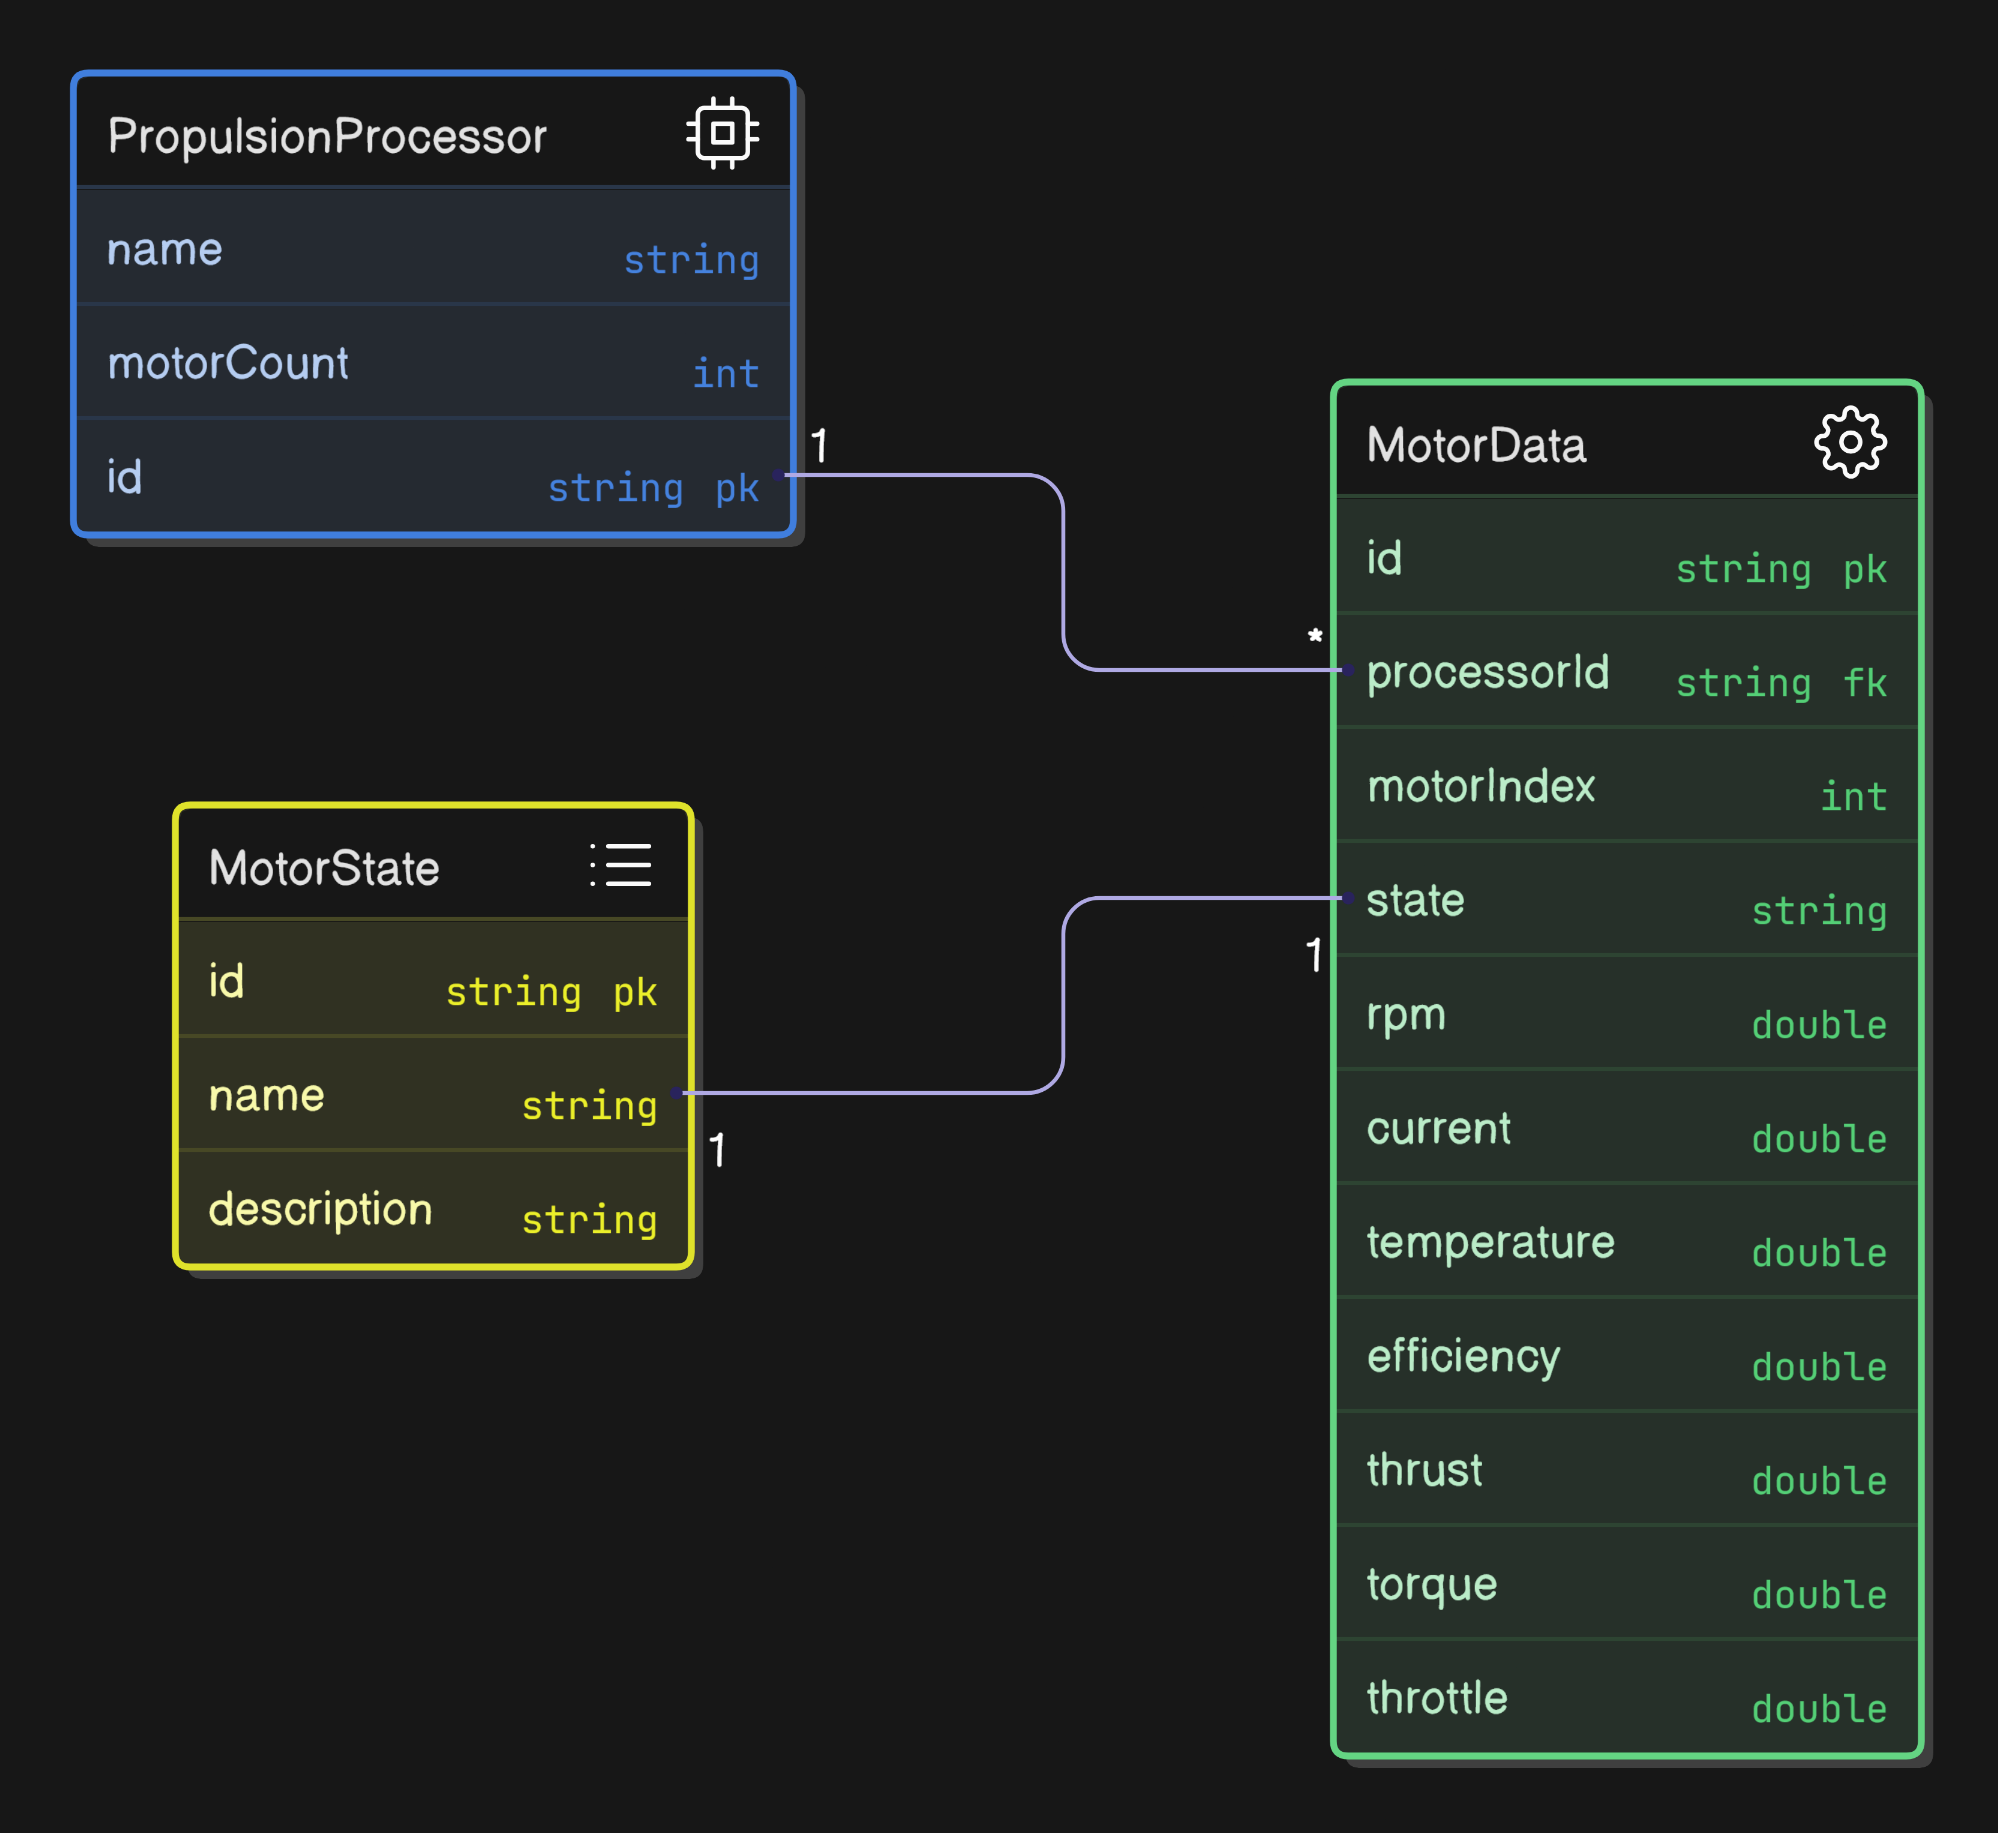
\includegraphics[width=0.8\textwidth,height=0.85\textheight,keepaspectratio]{images/08_ADD_motor_state_array.png}
\caption{\unclass Motor State Array}
\label{fig:motor_state_array}
\end{center}
\end{figure}

\subsection{\unclass Update Loop}\label{sec:PropUpdateLoop}

\begin{figure}[H]
\begin{center}
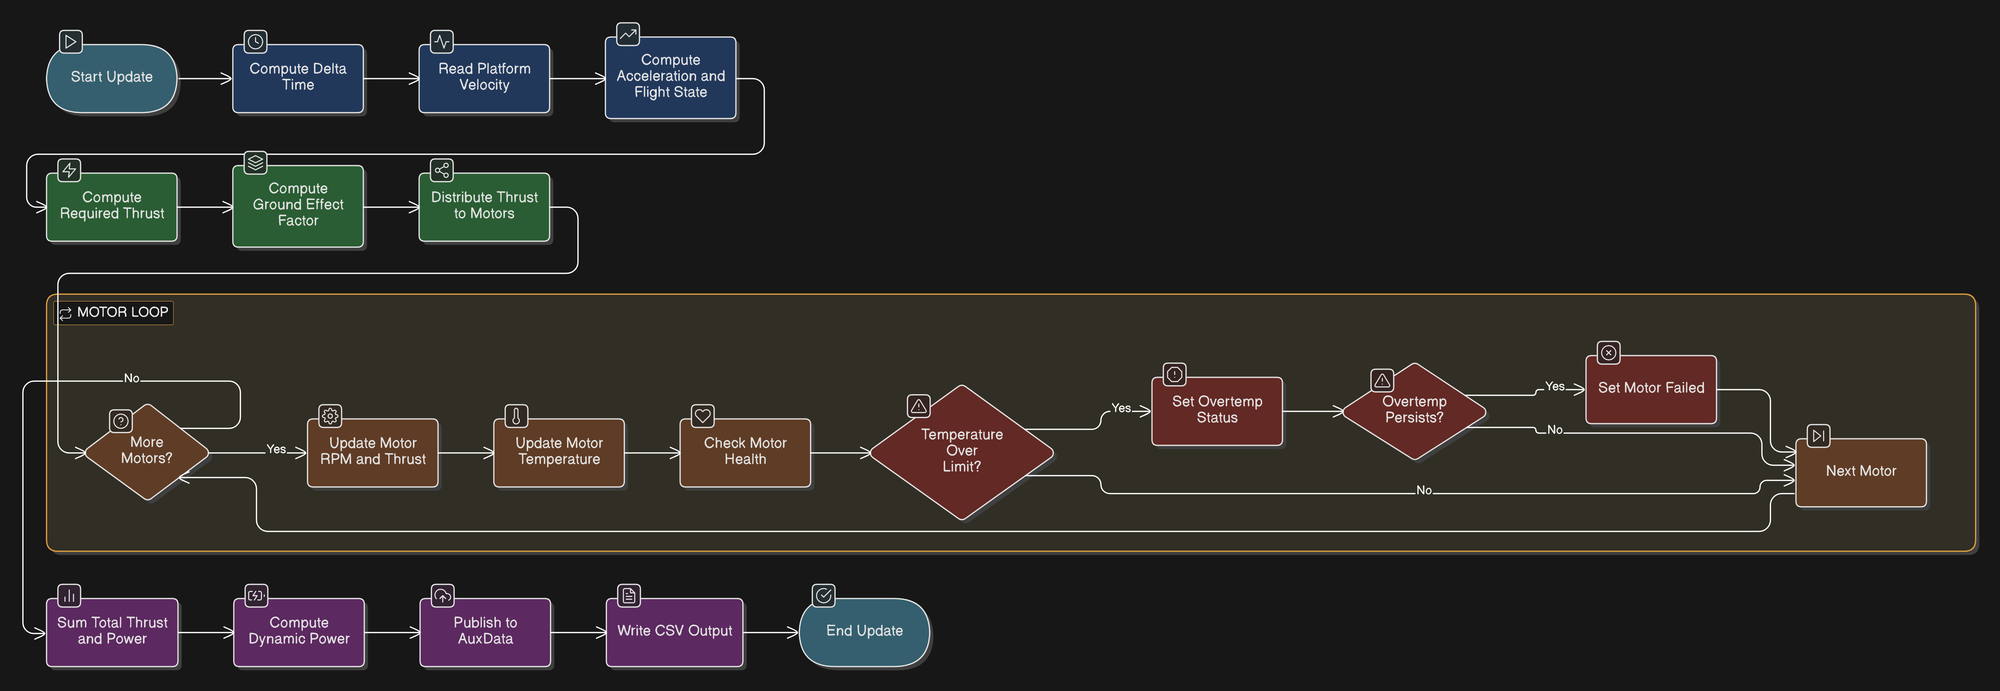
\includegraphics[width=\textwidth,height=0.85\textheight,keepaspectratio]{images/09_ADD_propulsion_update_loop.png}
\caption{\unclass Propulsion Update Loop}
\label{fig:propulsion_update_loop}
\end{center}
\end{figure}

\subsection{\unclass MotorState Machine}\label{sec:MotorStateMachine}

\begin{figure}[H]
\begin{center}
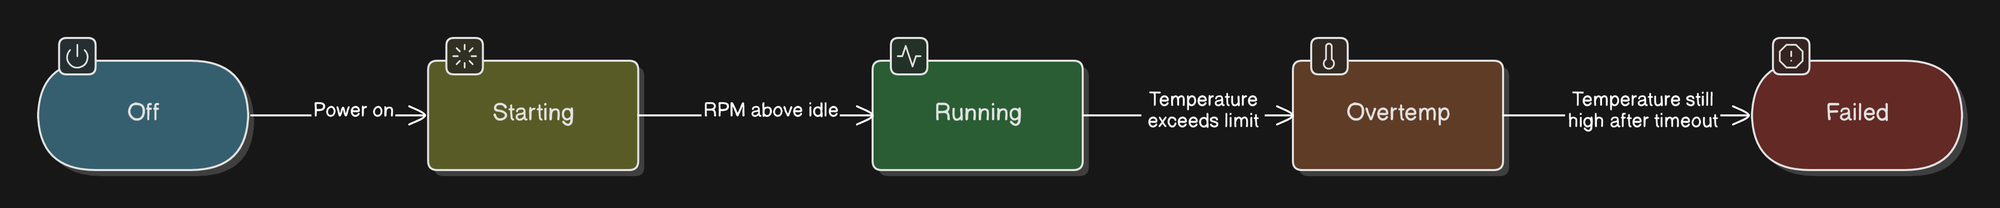
\includegraphics[width=0.8\textwidth,height=0.85\textheight,keepaspectratio]{images/10_ADD_motor_state_machine.png}
\caption{\unclass Motor State Machine}
\label{fig:motor_state_machine}
\end{center}
\end{figure}

\unclass Transitions are governed by motor temperature relative to the configurable thermal limit. A failed motor produces zero thrust and is excluded from thrust distribution.

\subsection{\unclass Public Interface Summary}\label{sec:PropPublicInterface}

\tableThrNow{\unclasslabel}{\unclass PropulsionProcessor Public Interface}{PropPublicInterface}
{l,2.5in}{l,1.5in}{l,2in}
{
	Method & Precondition & Expected Outcome \\
	\texttt{GetTotalThrust()} & After Update & Returns sum of all motor thrust [N] \\
	\texttt{GetTotalPower()} & After Update & Returns total electrical power [W] \\
	\texttt{GetOperationalMotorCount()} & Any time & Returns count of motors not in FAILED state \\
	\texttt{GetMotorData(index)} & 0 $\leq$ index $<$ NUM\_MOTORS & Returns reference to individual motor state \\
	\texttt{GetMaxMotorTemperature()} & After Update & Returns highest motor temperature [$^\circ$C] \\
	\texttt{FailMotor(index)} & Motor is RUNNING & Forces motor to FAILED state \\
	\texttt{GetThrustMargin()} & After Update & Returns available thrust margin [0--1] \\
}

\pagebreak

%%%%%%%%%%%%%%%%%%%%%%%%%%%%%%%%%%%%%%%%%%%%%%%%%%%%%%%%%%%%
%% SECTION 6: Component -- VRSProcessor
%%%%%%%%%%%%%%%%%%%%%%%%%%%%%%%%%%%%%%%%%%%%%%%%%%%%%%%%%%%%

\section{\unclass Component: VRSProcessor}\label{sec:VRSProcessor}

\subsection{\unclass Structural Overview}\label{sec:VRSOverview}

\unclass The VRSProcessor detects and models Vortex Ring State conditions by monitoring descent rate and forward speed. It extends \texttt{WsfProcessor}.

\unclass \textbf{Source files:}

\tableTwoNow{\unclasslabel}{\unclass VRS Source Files}{VRSSourceFiles}{l,2.5in}{l,3in}{
	File & Purpose \\
	\texttt{VRSProcessor.hpp} & Class declaration, VRSState enum \\
	\texttt{VRSProcessor.cpp} & Implementation \\
	\texttt{VRSRegistration.hpp} & Scenario extension \\
	\texttt{VRSPluginRegistration.cpp} & Plugin entry points \\
}

\unclass \textbf{Namespace}: \texttt{t150}

\subsection{\unclass VRS State Machine}\label{sec:VRSStateMachine}

\begin{figure}[H]
\begin{center}
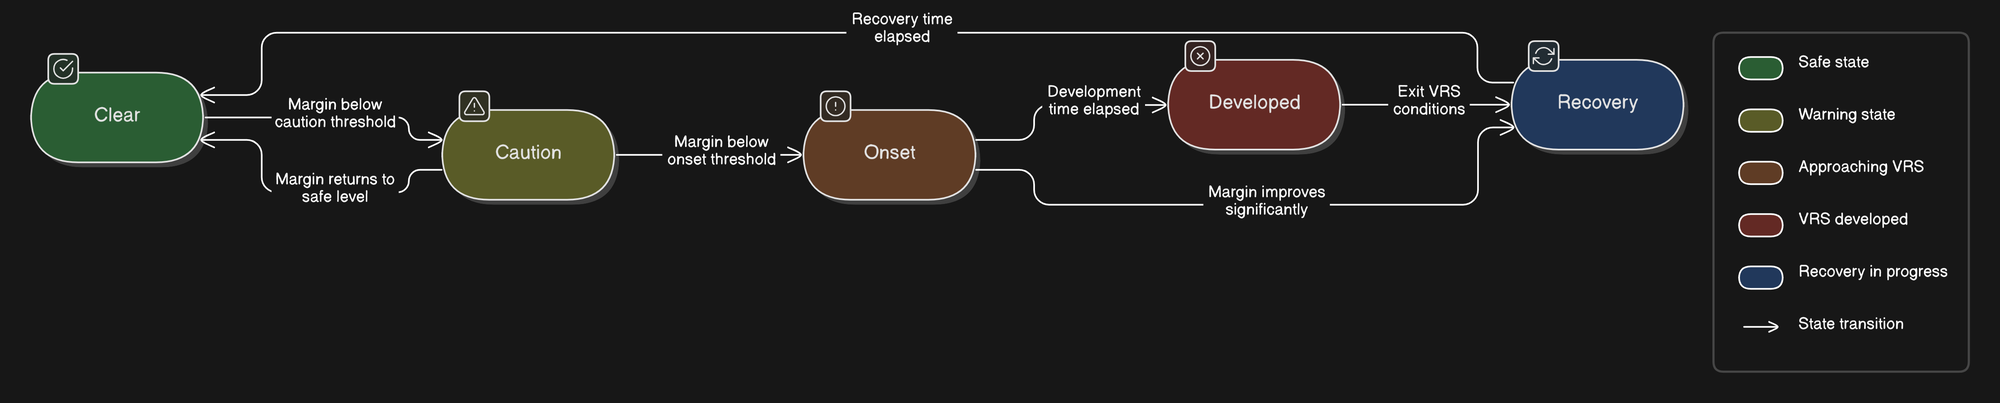
\includegraphics[width=0.8\textwidth,height=0.85\textheight,keepaspectratio]{images/11_ADD_vrs_state_machine.png}
\caption{\unclass VRS State Machine}
\label{fig:vrs_state_machine}
\end{center}
\end{figure}

\tableThrNow{\unclasslabel}{\unclass VRS State Descriptions}{VRSStateDescriptions}
{l,1in}{l,2.5in}{l,2.5in}
{
	State & Condition & Effect \\
	CLEAR & VRS margin $>$ caution threshold & No degradation (lift factor $= 1.0$) \\
	CAUTION & Margin between caution and onset thresholds & Warning issued, no degradation yet \\
	ONSET & Margin below onset threshold & Partial lift degradation begins \\
	DEVELOPED & Onset sustained for development time & Full lift and control degradation applied \\
	RECOVERY & Conditions improving & Gradual restoration of lift and control \\
}

\subsection{\unclass Velocity Reading}\label{sec:VRSVelocityReading}

\unclass The VRS processor reads descent rate and forward speed from the platform's mover state (via AFSIM's \texttt{WsfPlatform} API), not from AuxData. It calls the platform's velocity accessors to obtain NED velocity components, then derives descent rate (negative of down velocity) and horizontal speed.

\subsection{\unclass Public Interface Summary}\label{sec:VRSPublicInterface}

\tableThrNow{\unclasslabel}{\unclass VRSProcessor Public Interface}{VRSPublicInterface}
{l,2in}{l,1.5in}{l,2.5in}
{
	Method & Precondition & Expected Outcome \\
	\texttt{GetVRSState()} & After Update & Returns current VRSState enumeration \\
	\texttt{GetVRSMargin()} & After Update & Returns proximity to VRS [0--1], lower $=$ closer \\
	\texttt{GetLiftFactor()} & After Update & Returns lift multiplier [0--1], 1.0 $=$ no degradation \\
	\texttt{GetControlFactor()} & After Update & Returns control authority [0--1] \\
	\texttt{IsInVRS()} & After Update & Returns true if state $==$ DEVELOPED \\
	\texttt{GetTimeInState()} & After Update & Returns seconds in current state \\
}

\pagebreak

%%%%%%%%%%%%%%%%%%%%%%%%%%%%%%%%%%%%%%%%%%%%%%%%%%%%%%%%%%%%
%% SECTION 7: Component -- SlungLoadProcessor
%%%%%%%%%%%%%%%%%%%%%%%%%%%%%%%%%%%%%%%%%%%%%%%%%%%%%%%%%%%%

\section{\unclass Component: SlungLoadProcessor}\label{sec:SlungLoadProcessor}

\subsection{\unclass Structural Overview}\label{sec:SlungOverview}

\unclass The SlungLoadProcessor models a cable-suspended payload as a spherical pendulum. It computes swing dynamics, cable tension, and reaction forces that are published to AuxData for the mover to read. It extends \texttt{WsfProcessor}.

\unclass \textbf{Source files:}

\tableTwoNow{\unclasslabel}{\unclass Slung Load Source Files}{SlungSourceFiles}{l,2.5in}{l,3in}{
	File & Purpose \\
	\texttt{SlungLoadProcessor.hpp} & Class declaration, SlungLoadState enum \\
	\texttt{SlungLoadProcessor.cpp} & Implementation \\
	\texttt{SlungLoadRegistration.hpp} & Scenario extension \\
	\texttt{SlungLoadPluginRegistration.cpp} & Plugin entry points \\
}

\unclass \textbf{Namespace}: \texttt{t150}

\subsection{\unclass Pendulum Integration Loop}\label{sec:PendulumIntegration}

\unclass Each timestep, the processor executes:

\begin{figure}[H]
\begin{center}
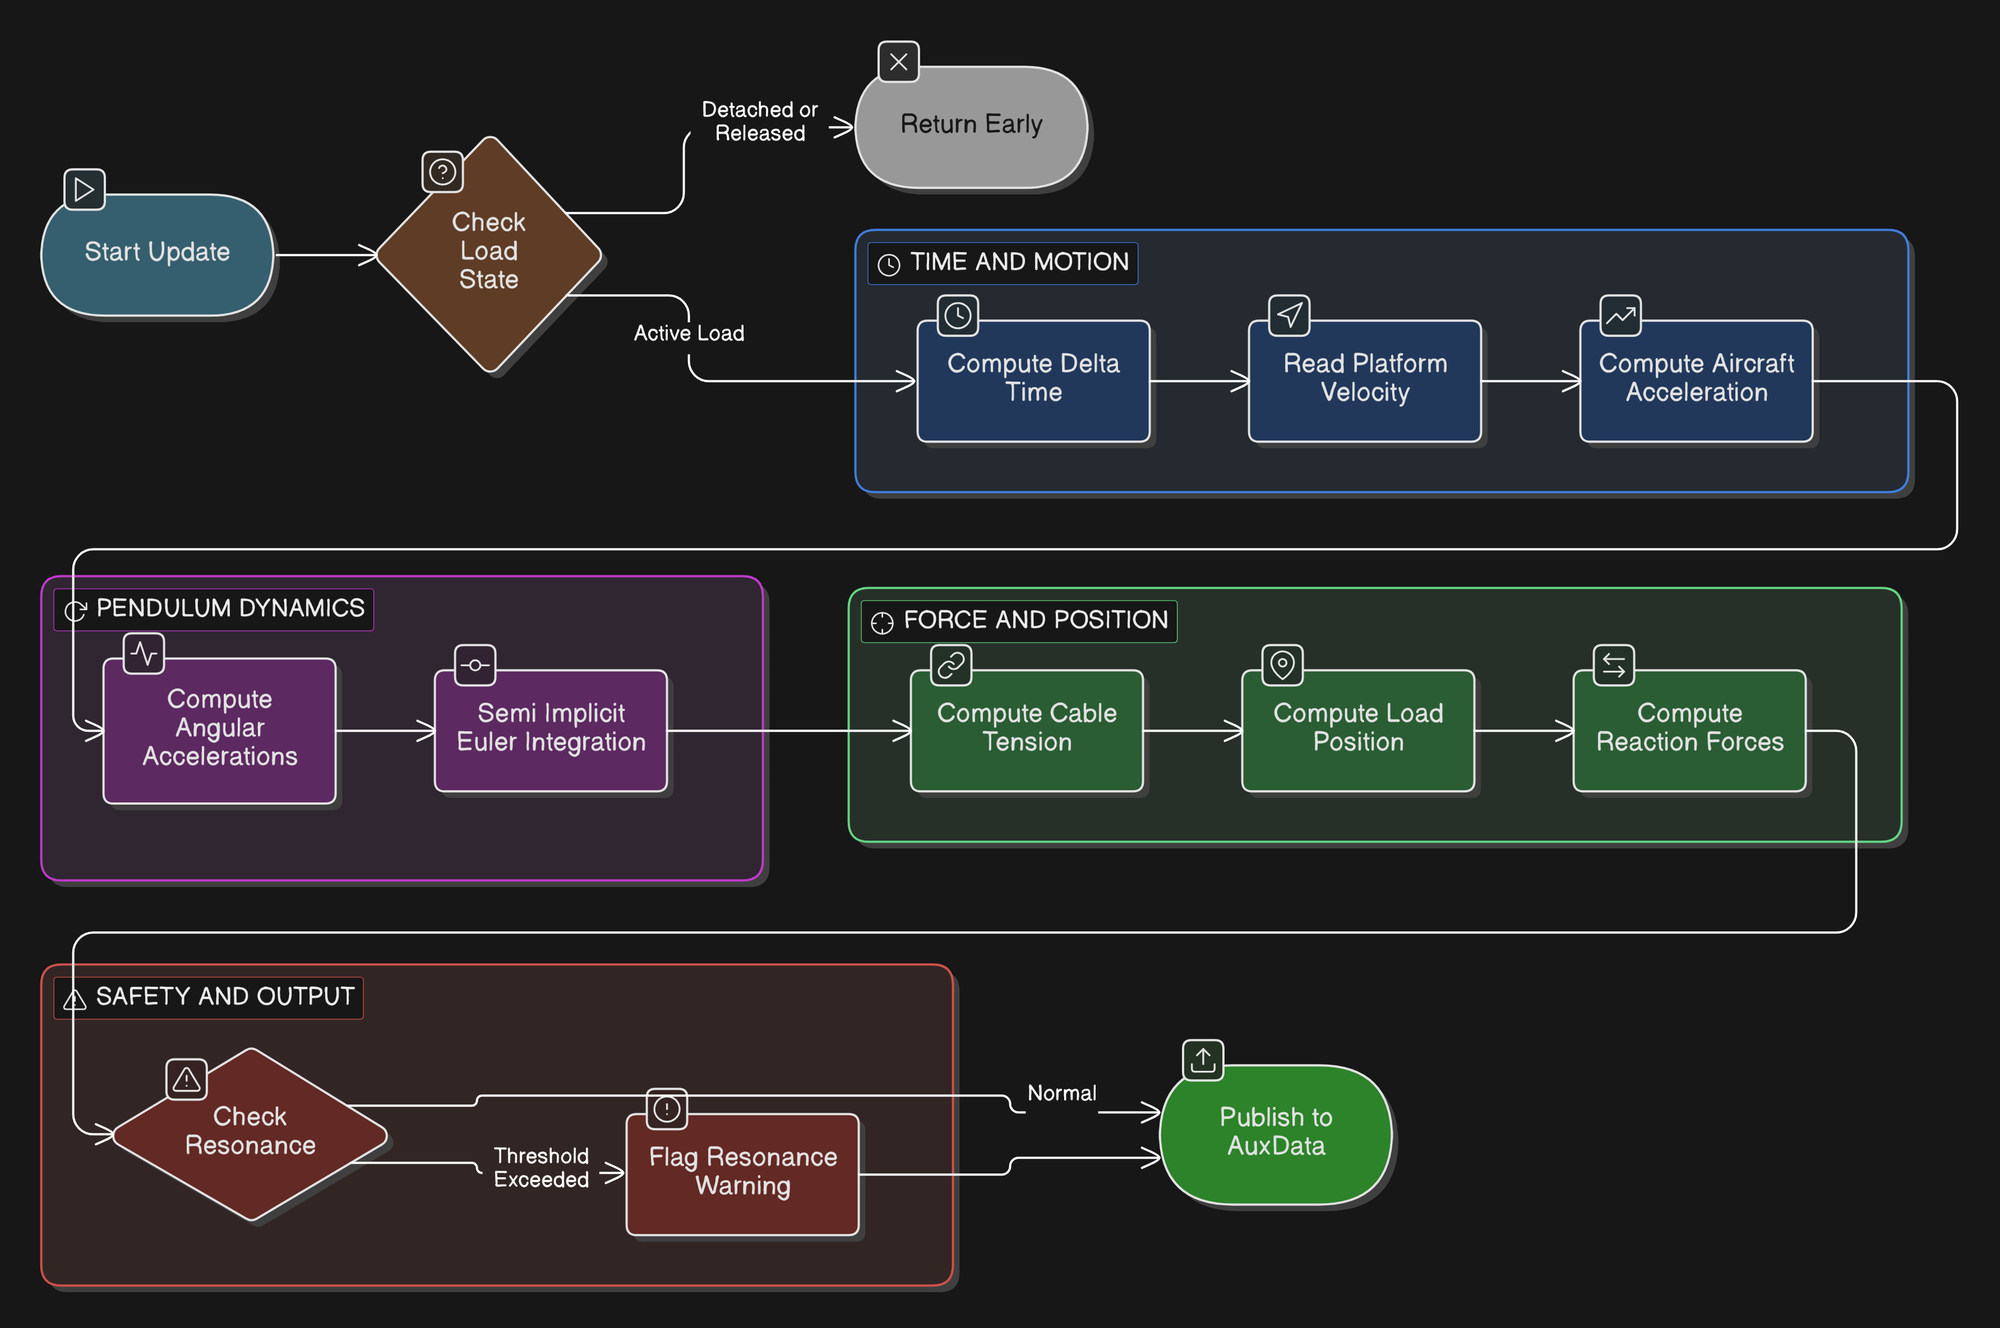
\includegraphics[width=\textwidth,height=0.85\textheight,keepaspectratio]{images/12_ADD_slung_load_integration_loop.png}
\caption{\unclass Slung Load Pendulum Integration Loop}
\label{fig:slung_load_integration_loop}
\end{center}
\end{figure}

\subsection{\unclass SlungLoad State Machine}\label{sec:SlungStateMachine}

\begin{figure}[H]
\begin{center}
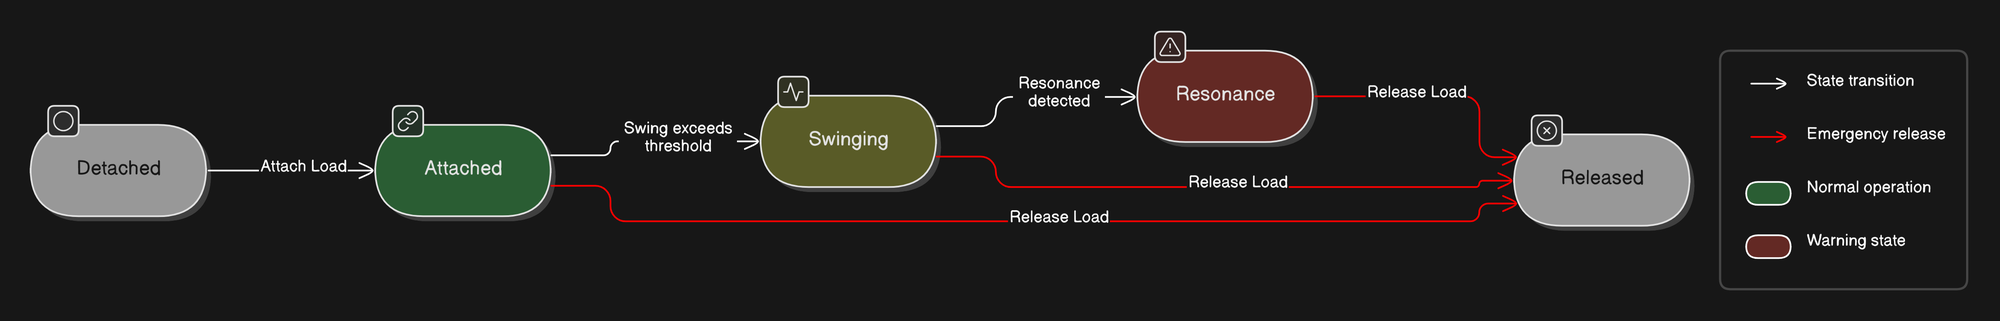
\includegraphics[width=0.8\textwidth,height=0.85\textheight,keepaspectratio]{images/13_ADD_slung_load_state_machine.png}
\caption{\unclass Slung Load State Machine}
\label{fig:slung_load_state_machine}
\end{center}
\end{figure}

\tableThrNow{\unclasslabel}{\unclass Slung Load State Descriptions}{SlungStateDescriptions}
{l,1in}{l,2.5in}{l,2.5in}
{
	State & Condition & Behavior \\
	DETACHED & No load & No dynamics computed \\
	ATTACHED & Load connected, small swing & Normal pendulum dynamics \\
	SWINGING & Swing angle $>$ threshold & Warning issued, dynamics continue \\
	RESONANCE & Measured frequency near natural frequency & Critical warning \\
	RELEASED & Load intentionally dropped & Forces zeroed, state frozen \\
}

\subsection{\unclass Force Coupling to Mover}\label{sec:ForceCoupling}

\unclass The slung load processor publishes \texttt{SLUNG\_FORCE\_X/Y/Z} to AuxData. The Rotorcraft6DOF mover reads these keys in its \texttt{ReadExternalForces()} method and adds them to the total force vector before integration. This creates a bidirectional coupling: aircraft motion drives pendulum dynamics (via acceleration), and pendulum forces affect aircraft motion (via AuxData).

\subsection{\unclass Public Interface Summary}\label{sec:SlungPublicInterface}

\tableThrNow{\unclasslabel}{\unclass SlungLoadProcessor Public Interface}{SlungPublicInterface}
{l,2in}{l,1.5in}{l,2.5in}
{
	Method & Precondition & Expected Outcome \\
	\texttt{AttachLoad(mass)} & State is DETACHED & Transitions to ATTACHED, sets load mass \\
	\texttt{ReleaseLoad()} & State is ATTACHED/ SWINGING/RESONANCE & Transitions to RELEASED, zeroes forces \\
	\texttt{GetSwingMagnitude()} & After Update & Returns RSS swing angle [rad] \\
	\texttt{GetCableTension()} & After Update & Returns cable tension [N] \\
	\texttt{GetLoadForceX/Y/Z()} & After Update & Returns reaction force components [N] \\
	\texttt{IsResonanceWarning()} & After Update & Returns true if resonance detected \\
}

\pagebreak

%%%%%%%%%%%%%%%%%%%%%%%%%%%%%%%%%%%%%%%%%%%%%%%%%%%%%%%%%%%%
%% SECTION 8: Design Decisions
%%%%%%%%%%%%%%%%%%%%%%%%%%%%%%%%%%%%%%%%%%%%%%%%%%%%%%%%%%%%

\section{\unclass Design Decisions}\label{sec:DesignDecisions}

\subsection{\unclass Decision Log}\label{sec:DecisionLog}

\begin{center}
\begin{longtblr}
	[
		caption={\unclass Design Decision Log},
		label={tab:DesignDecisionLog},
	]{
		colspec={|Q[valign=m,c,0.4in]|Q[valign=m,l,1.5in]|Q[valign=m,l,2in]|Q[valign=m,l,2in]|},
		hline{1-Z}={.5pt},
		cell{1}{1}={c=4}{halign=l},
		cell{Z}{1}={c=4}{halign=r},
		row{2}={bg=TableBlue,fg=white,halign=c},
		rowhead=2,
		rowfoot=1,
	}
	\unclasslabel & & &\\
	ID & Decision & Rationale & Alternatives Considered \\
	DD-01 & Extend WsfRouteMover rather than WsfMover & WsfRouteMover provides built-in route/waypoint management, arrival detection, and pause/resume. Extending WsfMover directly would require reimplementing all route logic. & WsfMover (rejected: too much route logic to reimplement) \\
	DD-02 & AuxData blackboard for inter-plugin communication & Decouples plugins; any subset can run independently. Plugins use fallback values when expected AuxData keys are absent. & Direct object references (rejected: build-time coupling); AFSIM message bus (rejected: higher complexity) \\
	DD-03 & Quaternion attitude representation & Avoids gimbal lock inherent in Euler angle integration. Quaternion normalization is computationally cheap. Euler angles are derived only for telemetry output. & Euler angles (rejected: gimbal lock at 90-deg pitch); rotation matrices (rejected: 9 elements vs 4) \\
	DD-04 & Custom math library (MathUtils.hpp) & AFSIM's built-in math (UtVec3) uses different conventions. A self-contained Vector3/Quaternion/Matrix3x3 library ensures NED consistency and avoids API breakage across AFSIM versions. & UtVec3/UtQuat (rejected: convention mismatch); Eigen (rejected: large dependency for plugin deployment) \\
	DD-05 & Per-plugin shared library & Each plugin can be deployed, updated, and tested independently. Scenario files load only the plugins needed. & Monolithic library (rejected: all-or-nothing deployment); header-only (rejected: AFSIM plugins must be shared libraries) \\
	DD-06 & First-order motor lag & Captures motor spin-up/spin-down dynamics with a single time constant parameter. Good fidelity-to-complexity ratio for engagement-level simulation. & Instantaneous response (rejected: unrealistic); second-order dynamics (rejected: added complexity with minimal fidelity gain) \\
	DD-07 & Semi-implicit Euler for pendulum integration & Unconditionally stable for the slung load pendulum, simple to implement. Energy dissipation from damping term prevents numerical divergence. & RK4 (considered: more accurate but pendulum damping makes Euler adequate); symplectic Euler (equivalent) \\
	DD-08 & Catmull-Rom splines for path interpolation & C1-continuous curves through waypoints without requiring user-specified tangents. Tension parameter provides tuning. Sliding 4-point window keeps memory bounded. & Linear interpolation (rejected: abrupt heading changes); B-splines (rejected: do not pass through control points); Bezier (rejected: require tangent specification) \\
	DD-09 & Configurable power source key & Battery processor can read power from any AuxData key, allowing it to pair with the propulsion processor, the 6DOF mover, or a custom source without code changes. & Hard-coded key (rejected: limits reuse); direct processor reference (rejected: coupling) \\
	DD-10 & \texttt{generate\_export\_header()} for DLL support & CMake's \texttt{GenerateExportHeader} module automatically generates the correct \texttt{\_\_declspec(dllexport)} / visibility macros for cross-platform builds. & Manual export macros (rejected: error-prone); WINDOWS\_EXPORT\_ALL\_SYMBOLS only (rejected: fragile with templates) \\
	\unclasslabel & & &\\
\end{longtblr}
\end{center}

\pagebreak

%%%%%%%%%%%%%%%%%%%%%%%%%%%%%%%%%%%%%%%%%%%%%%%%%%%%%%%%%%%%
%% SECTION 9: Installation and Build
%%%%%%%%%%%%%%%%%%%%%%%%%%%%%%%%%%%%%%%%%%%%%%%%%%%%%%%%%%%%

\section{\unclass Installation and Build}\label{sec:InstallBuild}

\subsection{\unclass Build System}\label{sec:BuildSystem}

\unclass The plugin suite uses CMake (minimum version 3.16) with the following structure:

\begin{figure}[H]
\begin{center}
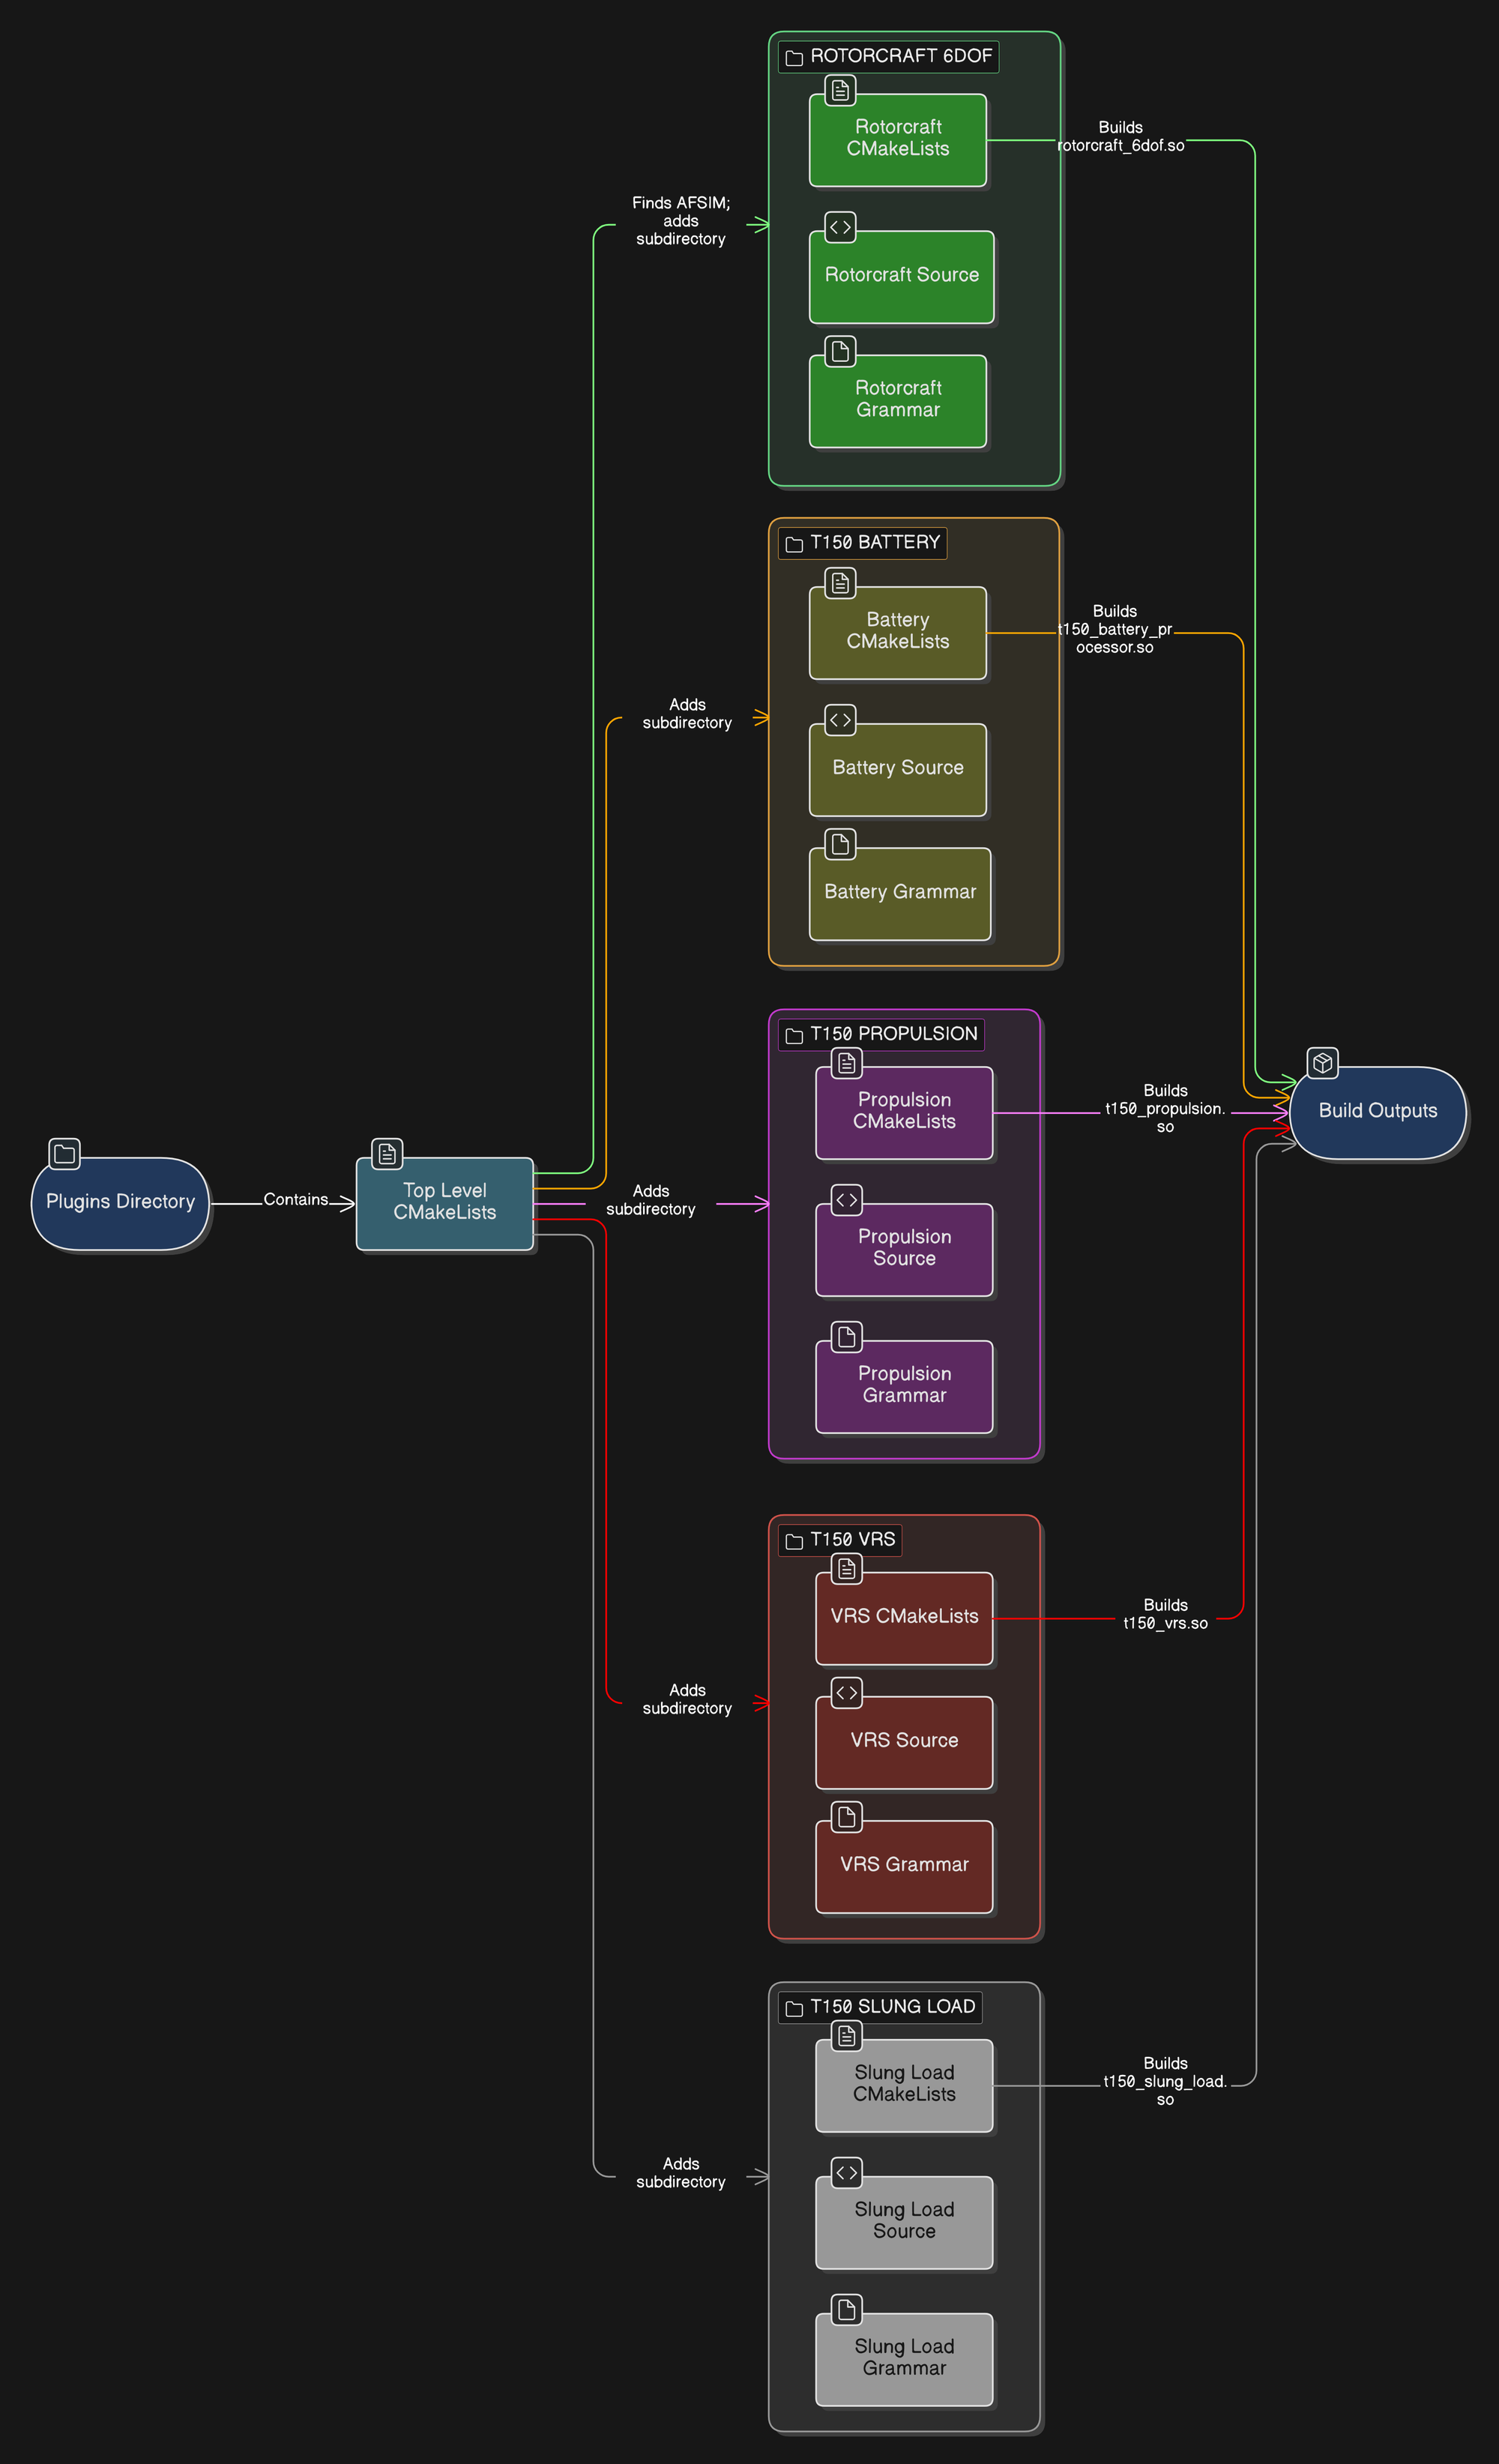
\includegraphics[width=0.8\textwidth,height=0.85\textheight,keepaspectratio]{images/14_ADD_build_directory_structure.png}
\caption{\unclass Build Directory Structure}
\label{fig:build_directory_structure}
\end{center}
\end{figure}

\subsection{\unclass CMake Configuration}\label{sec:CMakeConfig}

\unclass Each plugin's \texttt{CMakeLists.txt} follows the same pattern:

\begin{enumerate}
	\item \unclass Define PLUGIN\_NAME
	\item \unclass Glob source files (\texttt{*.cpp}, \texttt{*.hpp})
	\item \unclass Create shared library: \texttt{add\_library(\$\{PLUGIN\_NAME\} SHARED ...)}
	\item \unclass Generate export header: \texttt{generate\_export\_header(\$\{PLUGIN\_NAME\} ...)}
	\item \unclass Set include directories: \texttt{source/}, build dir, AFSIM includes
	\item \unclass Link \texttt{AFSIM::wsf}
	\item \unclass Set properties: \texttt{POSITION\_INDEPENDENT\_CODE}, \texttt{PREFIX ""}, \texttt{WINDOWS\_EXPORT\_ALL\_SYMBOLS}
	\item \unclass Install to platform-appropriate directory:
	\begin{itemize}
		\item Linux: \texttt{lib/wsf\_plugins/}
		\item Windows: \texttt{bin/mission\_plugins/}
	\end{itemize}
\end{enumerate}

\unclass The top-level \texttt{CMakeLists.txt} detects the AFSIM installation via \texttt{find\_package(afsim REQUIRED)} and sets the C++ standard to C++20 (AFSIM \afsimVersion{} requirement).

\subsection{\unclass Build and Install Scripts}\label{sec:BuildInstallScripts}

\unclass The project provides NGIC convenience scripts at the repository root:

\tableTwoNow{\unclasslabel}{\unclass Build and Install Scripts}{BuildInstallScripts}{l,2in}{l,4in}{
	Script & Purpose \\
	\texttt{ngic\_afsim\_build.sh} & Auto-detects AFSIM installation, runs CMake configure and build \\
	\texttt{ngic\_afsim\_install.sh} & Installs built plugins to AFSIM system directories (requires sudo) \\
}

\unclass \textbf{Build procedure (pseudocode):}

\begin{verbatim}
  cd plugins/
  mkdir -p build && cd build
  cmake .. -DAFSIM_ROOT=/opt/afsim2.2505
  cmake --build . --parallel
\end{verbatim}

\unclass \textbf{Install destinations:}

\tableThrNow{\unclasslabel}{\unclass Install Destinations}{InstallDestinations}
{l,1in}{l,2.5in}{l,2.5in}
{
	Platform & Plugin Directory & Grammar Directory \\
	Linux & \texttt{/opt/afsim2.2505/lib/wsf\_plugins/} & \texttt{/opt/afsim2.2505/bin/grammar/} \\
	Windows & \texttt{C:\textbackslash AFSIM\textbackslash afsim2.2505\textbackslash bin\textbackslash mission\_plugins\textbackslash} & \texttt{C:\textbackslash AFSIM\textbackslash afsim2.2505\textbackslash bin\textbackslash grammar\textbackslash} \\
}

\subsection{\unclass Compiler Requirements}\label{sec:CompilerRequirements}

\tableThrNow{\unclasslabel}{\unclass Compiler Requirements}{CompilerRequirements}
{l,1.5in}{l,2in}{l,2.5in}
{
	Compiler & Minimum Version & Platform \\
	GCC & 13.3 & Linux (AlmaLinux 9 WSL) \\
	MSVC & 2022 (v143) & Windows 11 \\
	CMake & 3.16 & Both \\
	C++ Standard & C++17 (CMake configured for C++20) & Both \\
}

\pagebreak

%%%%%%%%%%%%%%%%%%%%%%%%%%%%%%%%%%%%%%%%%%%%%%%%%%%%%%%%%%%%
%% SECTION 10: Sources and References
%%%%%%%%%%%%%%%%%%%%%%%%%%%%%%%%%%%%%%%%%%%%%%%%%%%%%%%%%%%%

\section{\unclass Sources and References}\label{sec:SourcesReferences}

\unclass Reference the UAM for a comprehensive list of sources used to develop this model. The following references were used in creating this ADD.

\tableTwoNow{\unclasslabel}{\unclass References}{ADDReferences}{c,0.5in}{l,5.5in}{
	Ref & Citation \\
	{[1]} & Department of Defense Instruction 5000.61, ``DoD Modeling and Simulation (M\&S) Verification, Validation, and Accreditation (VV\&A),'' current version. \\
	{[2]} & MIL-STD-3022, ``Documentation of Verification, Validation, and Accreditation (VV\&A) for Models and Simulations,'' current version. \\
	{[3]} & T-150 UAS AFSIM Plugin Suite -- Underlying Algorithms Model (UAM), Version 3.0, March 2026. \\
	{[4]} & AFSIM User's Guide, Version \afsimVersion{}, Air Force Research Laboratory, 2025. \\
	{[5]} & Johnson, W. \textit{Helicopter Theory}, Dover Publications, 1994. \\
	{[6]} & Leishman, J. G. \textit{Principles of Helicopter Aerodynamics}, 2nd ed., Cambridge University Press, 2006. \\
	{[7]} & Brand, A. et al. ``Vortex Ring State (VRS) Prediction,'' AIAA Paper, 2004. \\
	{[8]} & Cicolani, L. S. et al. ``Simulation of the Dynamics of Helicopter Slung Load Systems,'' NASA/TP-2009-215656, 2009. \\
	{[9]} & Tremblay, O. and Bhatt, A. ``Experimental Validation of a Battery Dynamic Model for EV Applications,'' \textit{World Electric Vehicle Journal}, Vol. 3, 2009. \\
	{[10]} & T-150 UAS System Specification, [PLACEHOLDER -- Document ID], current version. \\
	{[11]} & AFSIM Plugin Developer's Guide, Air Force Research Laboratory, 2025. \\
}

\pagebreak

%%%%%%%%%%%%%%%%%%%%%%%%%%%%%%%%%%%%%%%%%%%%%%%%%%%%%%%%%%%%
%% SECTION 11: Acronyms
%%%%%%%%%%%%%%%%%%%%%%%%%%%%%%%%%%%%%%%%%%%%%%%%%%%%%%%%%%%%

\section{\unclass Acronyms}\label{sec:Acronyms}

\tableTwoNow{\unclasslabel}{\unclass Acronyms}{ADDAcronyms}{l,1.5in}{l,4in}{
	Acronym & Definition \\
	ADD & Architecture Description Document \\
	AFSIM & Advanced Framework for Simulation, Integration, and Modeling \\
	AGL & Above Ground Level \\
	API & Application Programming Interface \\
	CG & Center of Gravity \\
	CMake & Cross-platform build system \\
	CW/CCW & Clockwise / Counter-Clockwise \\
	DLL & Dynamic Link Library \\
	DoD & Department of Defense \\
	DoDI & Department of Defense Instruction \\
	DOF & Degrees of Freedom \\
	ESC & Electronic Speed Controller \\
	GCC & GNU Compiler Collection \\
	GE & Ground Effect \\
	ISA & International Standard Atmosphere \\
	LOC & Lines of Code \\
	MSL & Mean Sea Level \\
	MSVC & Microsoft Visual C++ \\
	NED & North-East-Down (coordinate frame) \\
	NGIC & National Ground Intelligence Center \\
	OCV & Open-Circuit Voltage \\
	PID & Proportional-Integral-Derivative (controller) \\
	RPM & Revolutions Per Minute \\
	SOC & State of Charge \\
	UAS & Unmanned Aircraft System \\
	UAM & Underlying Algorithms Model \\
	UML & Unified Modeling Language \\
	VRS & Vortex Ring State \\
	VV\&A & Verification, Validation, and Accreditation \\
	WSF & Warfighter Simulation Framework \\
}

\newpage\label{mylastpage}

%%% - - -   UNCLASSIFIED   - - - %%%
